\RequirePackage{fix-cm}
\documentclass[smallextended,envcountsect]{svjour3}

\smartqed
\usepackage{amsmath,amssymb,mathtools}
\usepackage{array,booktabs}
\usepackage{graphicx}
\usepackage[section]{placeins}
\usepackage{enumitem}
\usepackage{microtype}
\setlength{\emergencystretch}{1em}
\usepackage{xcolor}
\usepackage[numbers,sort&compress]{natbib}
\usepackage[colorlinks=true,allcolors=blue]{hyperref}
\usepackage[nameinlink,noabbrev]{cleveref}
\hypersetup{
  pdftitle={A Solver-Independent, Fixed-Topology Linear-Work Endpoint Certificate for Sparse Reciprocal Transportation},
  pdfauthor={Long Li}
}
\journalname{Preprint}
% Suppress the publisher's unassigned manuscript-number box in the preprint.
\renewcommand{\makeheadbox}{}

\spnewtheorem{assumption}[theorem]{Assumption}{\bfseries}{\itshape}

\newcommand{\R}{\mathbb{R}}
\newcommand{\cA}{\mathcal{A}}
\newcommand{\E}{\mathbb{E}}
\newcommand{\one}{\mathbf{1}}
\newcommand{\diag}{\operatorname{diag}}
\newcommand{\cC}{\mathcal{C}}
\newcommand{\cD}{\mathcal{D}}
\newcommand{\cF}{\mathcal{F}}
\newcommand{\cG}{\mathcal{G}}
\newcommand{\cS}{\mathcal{S}}
\newcommand{\norm}[1]{\left\lVert#1\right\rVert}

% Release-bound empirical values.  The generating script and submission audit
% regenerate this file from the A42 confirmatory analyses.
% Generated by experiments.make_a42_results_macros; do not edit.
% Values are authorized only with the complete A42 submission audit.
\newcommand{\AFTwoSourceDigest}{774d0f112b4cb2df2e77357a64780e96e7e33f3dc46531ee9458d3d01b6d0c1e}
\newcommand{\AFTwoSourceFiles}{141}
\newcommand{\AFTwoAnalysisCount}{12}
\newcommand{\AFTwoDynamicRounds}{1050}
\newcommand{\AFTwoDynamicVGMSeconds}{0.105565}
\newcommand{\AFTwoDynamicDampedGMSeconds}{0.0722185}
\newcommand{\AFTwoDynamicVOverDamped}{1.46175}
\newcommand{\AFTwoDynamicVOverStepwise}{0.291082}
\newcommand{\AFTwoBasinRounds}{1050}
\newcommand{\AFTwoBasinPasses}{720}
\newcommand{\AFTwoEndpointAccepts}{1050}
\newcommand{\AFTwoVerifierSlope}{1.02575}
\newcommand{\AFTwoVerifierSlopeLow}{1.01259}
\newcommand{\AFTwoVerifierSlopeHigh}{1.03783}
\newcommand{\AFTwoVerifierLargestEdges}{10000000}
\newcommand{\AFTwoVerifierLargestBytesPerEdge}{51.6079}
\newcommand{\AFTwoSkewRecords}{60}
\newcommand{\AFTwoSkewSlope}{1.01528}
\newcommand{\AFTwoSkewPlanBytesPerInput}{10}
\newcommand{\AFTwoSkewPlanBoundBytesPerInput}{12}
\newcommand{\AFTwoSharpnessRecords}{210}
\newcommand{\AFTwoSignedInflationMedian}{1}
\newcommand{\AFTwoStructuralInflationMedian}{1}
\newcommand{\AFTwoGlobalInflationMedian}{1.89906e+07}
\newcommand{\AFTwoSharpEdgeOnlyAtTen}{49}
\newcommand{\AFTwoPipelineRecords}{180}
\newcommand{\AFTwoPipelineMeasurements}{135}
\newcommand{\AFTwoPipelineTimedAccepts}{135}
\newcommand{\AFTwoPipelineSlope}{1.13588}
\newcommand{\AFTwoPipelineLargestEdges}{3000000}
\newcommand{\AFTwoPipelineLargestGMSeconds}{9.31139}
\newcommand{\AFTwoPipelineCandidateShare}{0.79933}
\newcommand{\AFTwoPipelineVerifyShare}{0.0478034}
\newcommand{\AFTwoGenreCells}{10}
\newcommand{\AFTwoGenreOracleOverEqual}{0.924997}
\newcommand{\AFTwoGenreHistoricalOverEqual}{1.00034}
\newcommand{\AFTwoGenreHistoricalOverOracle}{1.08145}
\newcommand{\AFTwoGenreEqualOracleOverEqual}{0.918347}
\newcommand{\AFTwoGenrePopularityOracleOverEqual}{0.931694}
\newcommand{\AFTwoEstimatorOracleMSE}{0.923077}
\newcommand{\AFTwoEstimatorStaleOneMSE}{0.923219}
\newcommand{\AFTwoEstimatorStaleTwentyMSE}{0.929779}
\newcommand{\AFTwoEstimatorCoordinateMSE}{1.8018}
\newcommand{\AFTwoStrictScalingGMSeconds}{1.13563}
\newcommand{\AFTwoStrictScalingMedianSeconds}{0.454156}
\newcommand{\AFTwoStrictScalingPninetySeconds}{139.547}
\newcommand{\AFTwoStrictScalingPninetyfiveSeconds}{141.645}
\newcommand{\AFTwoStrictScalingMaxSeconds}{147.939}
\newcommand{\AFTwoStrictScalingOptimal}{75}
\newcommand{\AFTwoStrictScalingOverV}{10.3187}
\newcommand{\AFTwoMovieLensEdges}{1000209}
\newcommand{\AFTwoMovieLensStrictAccepts}{5}
\newcommand{\AFTwoIndependentReplays}{18}
\newcommand{\AFTwoQuotaOneOracleMSE}{0.996607}
\newcommand{\AFTwoQuotaOneStaleOneMSE}{0.996767}
\newcommand{\AFTwoQuotaOneStaleTwentyMSE}{0.998781}
\newcommand{\AFTwoQuotaOneCoordinateMSE}{1.97158}
\newcommand{\AFTwoQuotaTenOracleMSE}{0.854972}
\newcommand{\AFTwoQuotaTenStaleOneMSE}{0.855097}
\newcommand{\AFTwoQuotaTenStaleTwentyMSE}{0.865543}
\newcommand{\AFTwoQuotaTenCoordinateMSE}{1.64665}

% Derived from research/reviewer_obstacle_results_a43.json and the bound A43
% raw records.  These macros are descriptive; the registered tree-insensitivity
% gate failed and no recommendation-accuracy claim is authorized.
\newcommand{\AFThreeSourceHashShort}{e78292a27473}
\newcommand{\AFThreeTreeRecords}{576}
\newcommand{\AFThreeTreeCells}{144}
\newcommand{\AFThreeTreeDisagreements}{104}
\newcommand{\AFThreeTreePositive}{576}
\newcommand{\AFThreeTreeInputAccepts}{35}
\newcommand{\AFThreeTreeMaxConductanceAccepts}{126}
\newcommand{\AFThreeTreeMinConductanceAccepts}{22}
\newcommand{\AFThreeTreeRandomAccepts}{36}
\newcommand{\AFThreeTreeGapRatioMedian}{2.06\ensuremath{\times10^{7}}}
\newcommand{\AFThreeTreeGapRatioPninetyfive}{2.14\ensuremath{\times10^{8}}}
\newcommand{\AFThreeTreeInputCorrectionMedian}{0.01055}
\newcommand{\AFThreeTreeMaxConductanceCorrectionMedian}{0.002504}
\newcommand{\AFThreeTreeMinConductanceCorrectionMedian}{0.01859}
\newcommand{\AFThreeTreeRandomCorrectionMedian}{0.006360}
\newcommand{\AFThreeMovieRecords}{3}
\newcommand{\AFThreeMovieAccepts}{3}
\newcommand{\AFThreeMovieUsersA}{2,664}
\newcommand{\AFThreeMovieUsersB}{3,254}
\newcommand{\AFThreeMovieUsersC}{4,081}
\newcommand{\AFThreeMovieEdgesA}{35,959}
\newcommand{\AFThreeMovieEdgesB}{44,129}
\newcommand{\AFThreeMovieEdgesC}{54,567}
\newcommand{\AFThreeMovieGapA}{7.87\ensuremath{\times10^{-17}}}
\newcommand{\AFThreeMovieGapB}{1.02\ensuremath{\times10^{-21}}}
\newcommand{\AFThreeMovieGapC}{2.23\ensuremath{\times10^{-22}}}
\newcommand{\AFThreeMovieResidualA}{3.00\ensuremath{\times10^{-14}}}
\newcommand{\AFThreeMovieResidualB}{6.25\ensuremath{\times10^{-14}}}
\newcommand{\AFThreeMovieResidualC}{4.51\ensuremath{\times10^{-14}}}
\newcommand{\AFThreeMovieSecondsA}{0.154}
\newcommand{\AFThreeMovieSecondsB}{0.202}
\newcommand{\AFThreeMovieSecondsC}{0.279}

% Generated by research/a45/analyze.py from source-bound A45 records.
\newcommand{\AFivePortMatched}{15}
\newcommand{\AFiveWorkloadAccepted}{12}
\newcommand{\AFiveImprovementMin}{41.5}
\newcommand{\AFiveImprovementMax}{53.5}
\newcommand{\AFiveFrozenAccepted}{178}
\newcommand{\AFiveFrozenBuilds}{27}
\newcommand{\AFiveFrozenSeconds}{0.800}
\newcommand{\AFiveAlwaysAccepted}{216}
\newcommand{\AFiveAlwaysBuilds}{216}
\newcommand{\AFiveAlwaysSeconds}{1.943}
\newcommand{\AFiveRetryAccepted}{216}
\newcommand{\AFiveRetryBuilds}{66}
\newcommand{\AFiveRetrySeconds}{1.112}
\newcommand{\AFiveColdAccepted}{16}
\newcommand{\AFiveBoundaryAccepted}{10}
\newcommand{\AFiveInvalidAccepted}{0}
\newcommand{\AFiveSmallPortPass}{9}
\newcommand{\AFiveSmallPortVerify}{3.506}
\newcommand{\AFiveSmallTransferVerify}{0.008}
\newcommand{\AFiveSmallPortPipeline}{6.085}
\newcommand{\AFiveSmallCQPipeline}{0.827}
\newcommand{\AFiveSmallPortRSS}{219.910}
\newcommand{\AFiveSmallCQRSS}{68.551}
\newcommand{\AFiveMediumPortPass}{6}
\newcommand{\AFiveMediumPortVerify}{31.265}
\newcommand{\AFiveMediumTransferVerify}{0.012}
\newcommand{\AFiveMediumPortPipeline}{34.440}
\newcommand{\AFiveMediumCQPipeline}{1.019}
\newcommand{\AFiveMediumPortRSS}{1728.133}
\newcommand{\AFiveMediumCQRSS}{68.984}


% Identity, affiliation, funding, interests, and publication rights confirmed
% by the sole author on 6 September 2026. No ORCID or DOI has been invented.
\newcommand{\PaperAuthorList}{Long Li}
\newcommand{\PaperAuthorRunning}{Long Li}
\newcommand{\PaperInstitute}{Long Li\\
  Independent Researcher\\
  \email{lilong0228@gmail.com}}
\newcommand{\FundingStatement}{This research received no specific external
  grant from any funding agency in the public, commercial, or not-for-profit
  sectors.}
\newcommand{\CompetingInterestsStatement}{The author declares no competing
  financial or non-financial interests.}
\newcommand{\AuthorContributionsStatement}{Long Li is the sole author and is
  responsible for the research, software, analysis, and manuscript. The use
  of AI-assisted tools is disclosed below.}
\newcommand{\RepositoryStatement}{The public companion repository is
  \url{https://github.com/long-0228/certquota}, with the paper and release
  links at \url{https://long-0228.github.io/certquota/}. The dated preprint
  release is identified by the tag \texttt{preprint-2026-09-06} and its Git
  commit. The public package contains the core source, installation tests,
  independent checkers, and a separately hash-manifested archive of 90
  synthetic-problem proofs. The 24 MovieLens-derived proof objects checked
  locally are not redistributed under the dataset's permission requirement. It
  is a curated publication snapshot, not the complete historical local
  reviewer bundle. No archival DOI has yet been assigned.}


\title{A Solver-Independent, Fixed-Topology Linear-Work Endpoint Certificate
for Sparse Reciprocal Transportation}
\titlerunning{Fixed-Topology Endpoint Certification for Reciprocal Transport}
\author{\PaperAuthorList}
\authorrunning{\PaperAuthorRunning}
\institute{\PaperInstitute}
\date{6 September 2026}

\begin{document}
\maketitle

\begin{abstract}
Large sparse allocation solvers return floating-point candidates whose
marginals and optimality are only approximate.  This paper develops a
solver-independent endpoint certificate for sparse reciprocal transportation,
$\min_{z>0,Bz=\beta}\sum_e(c_ez_e+\mu_e/z_e)$ with $\mu_e>0$, directly on the
original sparse arrays.  From any finite candidate potential, a reciprocal KKT
allocation and canonical spanning-tree correction define an implicit exact-real
allocation.  A signed, outward-rounded replay either rejects or proves strict
positivity, exact feasibility for the represented marginals, and objective gap at most
$\varepsilon$.  Soundness is independent of the candidate generator under an
explicit binary64 and replay-ownership contract.  For a fixed candidate, the
bound converges to the exact recovery gap as interval widths vanish.  With
fixed-topology schedules, verification uses $O(m+n)=O(m)$ work and memory; each
$m$-input grouped plan stores exactly $m-g$ additions for $g$ nonempty groups.
CertQuota-V makes replay the sole authority over untrusted generators.
Evaluation covers certificate sharpness, adversarial degree skew, verifier-only
and complete-pipeline scaling, matched-accuracy independently checked conic
bounds, dynamic tree policies, hard starts, and budget decisions on
historical-only MovieLens workloads.
The result is a reusable, structure-specific verified numerical primitive: it
avoids an edgewise conic lift, does not trust solver status, and binds the
feasibility and gap claims to the same recovered allocation.
\keywords{certifying algorithms \and interval arithmetic \and convex network
flow \and sparse transportation \and primal recovery \and reproducible
numerical software}
\subclass{90C25 \and 90C35 \and 65G20}
\end{abstract}
\section{Introduction}

Sparse convex allocation appears in transportation, resource assignment, and
sampling.  At scale, a solver ordinarily returns a floating-point point, a
residual, and a status flag.  None alone establishes that the represented
allocation is strictly inside its domain, satisfies its marginals exactly, and
lies within a prescribed objective gap.  General verified-optimization
machinery can address broader models, but a structure-specific endpoint check
can be substantially smaller and can expose exactly which original data and
floating-point operations carry authority.

We develop such a check for the sparse reciprocal transportation problem
\begin{equation}
 P^\star=\inf_{z>0,\;Bz=\beta}P(z),\qquad
 P(z)=\sum_{e\in E}\left(c_ez_e+\frac{\mu_e}{z_e}\right),
 \quad \mu_e>0,
 \label{eq:problem}
\end{equation}
where $B$ is an oriented incidence matrix of a connected bipartite graph with
$m=|E|$ edges and $n$ vertices.  Throughout, $c$ is finite, every
$\mu_e>0$, and $\one^\top\beta=0$.  The global candidate solvers are designed
for instances having bipartite-sign marginals and a strictly positive feasible
point.  The endpoint soundness theorem does not assume an external feasibility
oracle: on acceptance, the recovered $Z>0$ itself discharges nonemptiness for
the represented instance.

The setting is deliberately narrower than general convex flow.  Newton and
interior methods for separable network objectives are classical
\citep{klincewicz1983,klincewicz1989}; specialized solvers exploit bipartite
normal equations \citep{castro2021huge,wright2023direct}; and modern theory
handles broader flow objectives in almost-linear time
\citep{chen2025maxflow}.  Certifying algorithms and rigorous optimization
postprocessing are established paradigms as well
\citep{mcconnell2011certifying,jansson2004convex,jansson2007rigorous}.  We ask a
different endpoint question: can an arbitrary finite candidate potential be
checked on the original sparse edge arrays, with no appeal to the generator's
status or stopping rule, while preserving support and using only linear work?

The difficulty is not writing a real-arithmetic dual bound.  The endpoint must
identify one positive exactly feasible primal object, prove the gap for that
same object, preserve a prescribed sparse support, and carry every inequality
through a finite replay without trusting a conic reduction or solver status.
Generic conic verification can represent the problem with one cone block per
edge. Earlier network-flow work already recovers primal feasibility from an
arbitrary Lagrangian dual vector \citep{marklund2008early}; candidate independence
alone is therefore not our distinction. The contribution here is a smaller
original-array, finite-arithmetic contract for this reciprocal structure. Its value is judged
as a reusable verification primitive and software interface, not as a new
transport objective.

Two identities make the answer possible.  First, a dual potential determines
an edgewise reciprocal KKT allocation.  Second, the residual of that allocation
can be routed uniquely over a fixed spanning tree.  The resulting correction
restores the marginals without introducing an off-support edge, and its exact
primal--dual gap is a sum of nonnegative edge terms.  Retaining the correction's
sign inside an outward-rounded replay turns those identities into a sharp
endpoint predicate: one accepted object simultaneously carries positivity,
exact-real feasibility, and $\varepsilon$-optimality.  Candidate generation and
authorization are therefore separate concerns.

One motivating application is variance-aware multi-model federated learning
(MMFL).  Each client makes one categorical decision among its eligible models,
while both client activation budgets and model participation targets are fixed
in expectation.  Conditional Horvitz--Thompson variance then produces the
reciprocal term and the two families of quotas produce the two marginals.  This
differs from formulations with client capacities and only one global
participation total \citep{zhang2025optimal}.  The application motivates the
objective and supplies a conditional-MSE endpoint; it is not needed by the
certificate theorem.

The paper answers three questions: what exact-real object an endpoint replay
authorizes, how a binary64 implementation encloses that object in linear work,
and whether separating a fast generator from strict authority remains useful at
sparse-graph scale.  Our contributions are:
\begin{enumerate}[leftmargin=*,itemsep=2pt]
 \item We define a canonical implicit allocation from any finite dual candidate
 and a support-preserving spanning-tree correction.  We prove that signed
 endpoint acceptance implies strict positivity, exact-real marginal
 feasibility, and objective gap at most $\varepsilon$, independently of how the
 candidate was generated.
 \item We give an executable original-array replay whose outward intervals bind
 the domain, tree correction, positivity, and primal--dual identity to the same
 recovered object; no edgewise conic lift or generator status carries
 authority.
 \item We prove fixed-candidate asymptotic completeness of the signed gap test
 and bound the irreducible conservatism of its sign-oblivious predecessor.  The
 distinction isolates interval-rounding overhead from loss caused by discarding
 correction signs.
 \item We give a fixed-DAG binary64 realization with explicit rounding and
 ownership assumptions.  On a fixed topology it uses $O(m+n)=O(m)$ work and
 memory.  Each $m$-input active-frontier grouped reduction stores exactly
 $m-g$ addition nodes for $g$ nonempty groups, even under arbitrarily skewed
 degrees.  A self-contained content-bound bundle lets a fresh process
 reconstruct all replay inputs and issue a new authoritative decision. A
 separate integer/rational checker evaluates the original primal and dual
 objectives without importing the production verifier.
 \item We implement the generate--certify--repair separation in CertQuota-V and
 evaluate soundness gates, sharpness, adversarial storage, verifier-only and
 complete-pipeline scaling, dynamic warm starts, named strict pipelines,
 independently replayed conic candidates, and conditional-MSE sampling on
 synthetic and real sparse supports.  A separately preregistered amendment
 quantifies tree-choice sensitivity on identical candidates and exercises
 prospective MovieLens inputs that never inspect post-cutoff ratings. An
 exploratory revision adds matched-accuracy, independently witnessed conic
 comparisons and an explicit rational-allocation budget decision interface.
 \item As one motivating reduction, we specialize conditional
 Horvitz--Thompson variance to independent categorical MMFL decisions and obtain
 the reciprocal objective under two-sided \emph{expected} quotas.  This
 application is not required by the endpoint theorem.
\end{enumerate}

\paragraph{Claim boundary.}
The new object is the endpoint contract, not the reciprocal objective, Newton
method, Laplacian Hessian, tree routing primitive, or general idea of posterior
certification.  Runtime comparisons apply only to the named implementations,
representation, hardware, and warm-start protocol in \cref{sec:experiments};
they do not rank all transportation or verified-optimization solvers.
Candidate-generator independence is a soundness statement about accepted
outputs, not a speed claim or an adversarial process-isolation guarantee: a
generator may supply arbitrary values and status but may not mutate verifier
inputs, code, private capabilities, or floating-point controls during replay.
The MMFL studies measure analytic conditional scheduler MSE, not trained-model
accuracy, fairness, or time to target.

\section{MMFL sampling under two-sided expected quotas}
\label{sec:mmfl}

Let $\cC$ be clients, $\cS$ models, and
$E\subseteq\cC\times\cS$ the sparse eligibility graph.  In one round, client
$i$ makes one categorical decision: it trains model $s$ with probability
$p_{is}>0$ or is idle.  The expected quotas are
\begin{equation}
 \sum_{s:(i,s)\in E}p_{is}=r_i,\quad 0<r_i\le1,
 \qquad
 \sum_{i:(i,s)\in E}p_{is}=d_s>0,
 \qquad \sum_i r_i=\sum_s d_s.
 \label{eq:quotas}
\end{equation}
We assume the sparse support admits a strictly positive allocation
$p^\circ>0$ satisfying these equalities.
Thus the row constraint enforces at most one job per client, while $d_s$ is a
model participation target only in expectation.  Requiring exact integer column
counts in every round needs dependent rounding and a different covariance
analysis \citep{gandhi2006rounding}.

For a finite represented instance, $(r,d)$ in \cref{eq:quotas} follows the
reduced-root convention of \cref{sec:recovery}: every client quota and every
non-root model quota is retained as its exact represented value, while the
distinguished model quota is defined by exact balance.  An independently
supplied binary64 value for that root quota is diagnostic only.  Thus every
``exact feasibility'' statement below refers to this represented quota vector,
not to two potentially inconsistent floating-point totals.

Let $u_{is}\in\R^k$ be the prospective local update and
$\alpha_{is}\ge0$ its aggregation weight.  To state the oracle objective
without anticipating unobserved randomness, define
$\cA_t:=\sigma(\cF_t,\{u_{is},\alpha_{is}:(i,s)\in E\})$.  The probabilities
$p_{is}$ are $\cA_t$-measurable.  Conditional on $\cA_t$, client decisions are
independent across clients and, for every $(i,s)\in E$,
$\Pr(Z_{is}=1\mid\cA_t)=p_{is}$; client $i$ is idle with probability $1-r_i$.
With $Z_{is}$ the selection indicator, define
\begin{equation}
 U_s=\sum_{i:(i,s)\in E}\alpha_{is}u_{is},\qquad
 \widehat U_s=\sum_{i:(i,s)\in E}
 \frac{Z_{is}\alpha_{is}}{p_{is}}u_{is}.
 \label{eq:ht}
\end{equation}

\begin{theorem}[Conditional Horvitz--Thompson variance identity]
\label{thm:mmfl}
Under the conditional inclusion probabilities and cross-client independence
specified above,
$\E[\widehat U_s\mid\cA_t]=U_s$ and
\begin{equation}
 \E\!\left[\norm{\widehat U_s-U_s}_2^2\mid\cA_t\right]
 =\sum_{i:(i,s)\in E}\alpha_{is}^2\norm{u_{is}}_2^2
 \left(\frac1{p_{is}}-1\right).
 \label{eq:variance}
\end{equation}
For model weights $\omega_s>0$, edge costs $\bar c_{is}\ge0$, and
$\gamma\ge0$, the weighted
sum of \cref{eq:variance} plus
$\gamma\E[\sum_{(i,s)\in E}\bar c_{is}Z_{is}\mid\cA_t]$ differs by a constant from
\begin{equation}
 \min_{p>0}\sum_{(i,s)\in E}
 \left(\frac{\mu_{is}}{p_{is}}+c_{is}p_{is}\right)
 \quad\text{s.t. \cref{eq:quotas}},
 \label{eq:mmfl-transport}
\end{equation}
where $\mu_{is}=\omega_s\alpha_{is}^2\norm{u_{is}}_2^2$ and
$c_{is}=\gamma\bar c_{is}$.
\end{theorem}

The proof is in \cref{app:mmfl}.  The exact identification with
\cref{eq:problem} requires
$\alpha_{is}\norm{u_{is}}_2>0$ on every declared edge.  We therefore define the
studied instance only after choosing a support on which $\mu_{is}>0$.  A
zero-weight eligibility relation lies outside that instance class: removing it
is an application-level change of support that can alter the feasible set, and
replacing it by a positive floor defines a surrogate objective.  Neither
operation is an exact numerical preprocessing rule for \cref{eq:problem}.

Exact update norms are also not normally known before scheduling.  We therefore
distinguish a nondeployable current-norm oracle from stale-norm and coordinate
proxies; a proxy allocation is optimal only for the surrogate weights supplied
to it.  This statistical limitation is separate from the numerical validity of
an accepted allocation.  A second distinction concerns representation: the
endpoint certificate below binds an implicit exact-real allocation, whereas a
conditional-MSE value computed from an emitted binary64 materialization belongs
to that finite vector.  The latter must be used consistently as both the
categorical inclusion law and the Horvitz--Thompson denominator; certificate
acceptance alone does not verify a sampler implementation.
\section{Dual candidate and exact-real tree recovery}
\label{sec:recovery}

Orient every edge from the client side to the model side, so $Bz=\beta=(r,-d)$.
For the theorem, let $v_0$ be a distinguished root.  The mathematical input is
the $n-1$ vector of independent binary64 quotas
$\bar\beta_{V\setminus\{v_0\}}$.  It retains those components as exact dyadics
and defines the root in exact real arithmetic by
\begin{equation}
 \beta_v:=\bar\beta_v\ (v\ne v_0),\qquad
 \beta_{v_0}:=-\sum_{v\ne v_0}\bar\beta_v,\qquad
 \Delta_{\rm root}:=\beta_{v_0}-\bar\beta_{v_0}.
 \label{eq:root}
\end{equation}
The recommended public constructor accepts only those $n-1$ independent values
and derives the root.  For backward compatibility, the full-vector constructor
fixes $v_0=n-1$, rejects nonfinite entries and a declared imbalance larger than
$10^{-9}\max\{1,\norm{\bar\beta}_1\}$, then stores the supplied root, an
\texttt{fsum}-based binary64 representative of the implied root, and a rounded
adjustment diagnostic $\widehat\Delta_{\rm root}$.  That compatibility value is
not an independent constraint.  The exact-real
$\Delta_{\rm root}$ in \cref{eq:root} is a mathematical definition reconstructed
from the independent entries during strict replay; it is not the stored
diagnostic.  The constructor does not decide general sparse transportation
feasibility.  Experimental generators numerically seed quotas from a positive
binary64 planted flow, but its rounded marginals are not asserted to equal
$Bx$ in exact-real arithmetic after the represented-root convention is imposed.
For every reported accepted instance, endpoint recovery itself supplies a
strictly positive exactly feasible $Z(P,y,T)$.  Other violations may lead only
to input rejection, certificate rejection, or explicit solver failure, never
to a strict accepted allocation.  All strict claims refer
to $\beta$ in \cref{eq:root}, not to the independently rounded vector
$\bar\beta$.
Operationally, the strict replay need not materialize the generally
non-binary64 root quota: it computes every non-root residual interval and
defines the root residual interval as the directed negative sum of those
intervals.  This is algebraically equivalent to the exact-real root convention.

For any stored candidate potential $y$, interpreted as an exact dyadic vector,
set
\begin{equation}
 q(y)=c-B^\top y,\qquad
 x_e(y)=\sqrt{\mu_e/q_e(y)},\qquad
 g(y)=Bx(y)-\beta.
 \label{eq:dual-state}
\end{equation}
When $q>0$, a dual lower bound is
\begin{equation}
 D(y)=\beta^\top y+2\sum_e\sqrt{\mu_eq_e(y)}.
 \label{eq:dual}
\end{equation}
Fix a spanning tree $T$.  Because $g$ is exactly balanced under
\cref{eq:root}, there is a unique tree-supported flow $h_T(y)$ satisfying
$Bh_T(y)=-g(y)$.  Computing a balanced flow on a tree is classical
\citep{ahuja1993network}; our use combines that routing primitive with the
reciprocal primal--dual identity and an executable outward-rounded certificate.
Define the canonical recovered object
\begin{equation}
 Z(P,y,T):=x(y)+h_T(y).
 \label{eq:implicit-z}
\end{equation}
This is an \emph{implicit exact-real allocation}.  It is represented by the
problem, candidate, tree, and certificate.  A downstream binary64 array
$\widehat z$ materializes the same formula numerically, but it is not asserted
to satisfy $B\widehat z=\beta$ bit for bit; its measured marginal residual is
always reported.

\section{Candidate-generator-independent endpoint verification}
\label{sec:verifier}

The authoritative verifier uses outward rounding to prove: (i) $q_e>0$;
(ii) lower bounds $\ell_e\le x_e(y)$; (iii) signed enclosures
$H_e=[\underline h_e,\overline h_e]\ni h_{T,e}(y)$; (iv) lower
bounds
\[
 \underline z_e:=\operatorname{down}(\ell_e+\underline h_e)>0
 \quad(e\in T)
\]
on the recovered allocation; and (v), with
$a_e:=\max\{|\underline h_e|,|\overline h_e|\}$,
\begin{equation}
 \Gamma_U:=\operatorname{up}\!\sum_{e\in T}
 \frac{\mu_ea_e^2}{\ell_e^2\underline z_e}\le\varepsilon.
 \label{eq:gamma}
\end{equation}
Non-tree correction coordinates are exactly zero.  The operation
$\operatorname{up}$ denotes an outward upper evaluation of the complete
reduction DAG, not merely a final rounded sum.

\paragraph{\textnormal{\textsc{EndpointVerify}}$(P,y,T,\varepsilon)$.}
The authoritative routine is the following fixed decision procedure.
\begin{enumerate}[leftmargin=*,itemsep=1pt]
 \item Validate dimensions, finite inputs, $\mu>0$, the root convention, and
 that $T$ spans the declared graph; otherwise do not authorize a return.  The
 low-level API may raise on malformed input.
 \item Evaluate outward intervals for every slack $q_e$; reject unless each
 lower endpoint is positive.  Evaluate intervals for $x$ and for the grouped
 residual $g=Bx-\beta$ using the precompiled reduction DAGs.
 \item Route the residual interval over $T$ to enclose the unique tree flow
 $f_T$ satisfying $Bf_T=g$, retain the signed enclosure
 $H_e=-F_e$ for $h_T=-f_T$, and reject unless every outward lower bound
 $\underline z_e=\operatorname{down}(\ell_e+\underline h_e)$ is positive.
 \item Evaluate the complete outward gap bound \cref{eq:gamma}.  Return
 \textsc{accept} exactly when $\Gamma_U\le\varepsilon$; otherwise return
 \textsc{reject}.  The logical acceptance trace contains
 $(P,y,T,\varepsilon,\Gamma_U,
 \{\ell_e,\underline h_e,\overline h_e,\underline z_e\})$.  The software returns an
 immutable replay key and compact summary rather than retaining both full
 edgewise interval arrays.
\end{enumerate}
Every exceptional arithmetic event is a rejection.  A binary64 materialization
may accompany an accepted tuple, but it is not the object authorized by this
procedure.  \textsc{SolveVerifyRepair} catches low-level exceptions and records
an explicit failed attempt with no allocation; the compact result does not
retain a primitive-level rejection reason code.  \Cref{app:ieee-predicate}
gives the primitive-level replay.

\begin{theorem}[Solver-independent endpoint soundness]
\label{thm:soundness}
Let $P$ be a validated represented instance of \cref{eq:problem}: its declared
graph is connected, its arrays are finite with $\mu_e>0$, and its marginals use
the reduced-root convention \cref{eq:root}.  Let $T$ be a validated spanning
tree of that graph, let $0<\varepsilon<+\infty$, and let $y$ be any finite
candidate array.  Under the execution contract in
\cref{assump:ieee-execution}, if the authoritative verifier accepts
$(P,y,T,\varepsilon)$, then $Z(P,y,T)$ is strictly positive,
$BZ(P,y,T)=\beta$ in exact-real arithmetic, and
\begin{equation}
 P(Z(P,y,T))-P^\star\le\Gamma_U\le\varepsilon.
 \label{eq:sound-gap}
\end{equation}
The conclusion is independent of how accurately, deterministically, or
successfully $y$ was generated, subject to the replay ownership and arithmetic
contract.
\end{theorem}

\begin{proof}
The executable-to-real bridge is \cref{lem:ieee-inclusion}: on every accepting
replay, each interval used below contains its exact-real DAG value.  The domain
 bounds therefore make $x(y)$ positive.  On a tree edge,
 $x_e+h_e\ge\ell_e+\underline h_e\ge\underline z_e>0$; non-tree entries
 remain $x_e>0$.  By construction,
$B(x+h_T)=\beta+g-g=\beta$.  Thus acceptance itself supplies a strictly
positive feasible point.  In particular, for every left vertex $i$,
\[
 \beta_i=\sum_{e\ni i}Z_e>0.
\]
Consequently every $\widetilde z\ge0$ with $B\widetilde z=\beta$ satisfies
$0\le\widetilde z_{is}\le\beta_i$; the nonnegative feasible closure is
therefore nonempty and compact.  Extending $P$ by $+\infty$ whenever an edge
coordinate is zero, the reciprocal barrier gives attainment in the positive
interior, and strict convexity gives uniqueness.  For every positive feasible
$u$, coordinatewise minimization of the Lagrangian gives $P(u)\ge D(y)$, so in
particular $P^\star\ge D(y)$.  For $z=x+h_T$, feasibility and
$q_e=\mu_e/x_e^2$ give
\begin{align}
 P(z)-D(y)
 &=\sum_e\left(q_ez_e+\frac{\mu_e}{z_e}
              -2\sqrt{\mu_eq_e}\right) \\
 &=\sum_e\frac{\mu_eh_e^2}{x_e^2(x_e+h_e)}.
 \label{eq:gap-identity}
\end{align}
 Weak duality and the certified inequalities bound each nonzero term by the
 corresponding summand of \cref{eq:gamma}: its numerator contains $h_e^2$,
 while $x_e\ge\ell_e$ and $x_e+h_e\ge\underline z_e$.  The outward reduction contains their
 sum.  No step uses how $y$ was obtained.
\end{proof}

\begin{proposition}[Fixed-DAG interval continuity and fixed-candidate completeness]
\label{prop:asymptotic-completeness}
Fix $(P,y,T)$ with $q(y)>0$ and $Z(P,y,T)>0$.  Consider interval
evaluations of the same finite expression DAG, indexed by $k$.  For every
exact-real node value $v$, require its enclosure $I_{k,v}$ to satisfy
$v\in I_{k,v}$ and $\operatorname{diam}(I_{k,v})\to0$.  For all sufficiently
large $k$, the domain and positivity denominators are positive; let
$\Gamma_{U,k}$ denote the resulting upper gap endpoint.  Then
$\Gamma_{U,k}\ge G(y,T)$ for every such $k$ and
$\Gamma_{U,k}\to G(y,T)$, where
\begin{equation}
 G(y,T):=P(Z(P,y,T))-D(y)
 =\sum_{e\in T}\frac{\mu_eh_e^2}{x_e^2(x_e+h_e)}.
 \label{eq:exact-recovery-gap}
\end{equation}
Consequently, if $G(y,T)<\varepsilon$, every sufficiently narrow member of
this interval-evaluation family accepts.  A fixed binary64 replay remains
deliberately fail-closed and may
reject such a candidate.  No nesting or monotonic decrease of the interval
endpoints is assumed.
\end{proposition}

The sign retention is essential for this conclusion.  The legacy
sign-oblivious predicate first requires $x_e-|h_e|>0$ on every tree edge.
If $\rho:=\max_{e\in T}|h_e|/x_e\ge 1$, that positivity gate rejects
(equivalently, set $\Gamma_{\rm abs}=+\infty$).  Only when $\rho<1$ does its
limiting bound equal
\begin{equation}
 \Gamma_{\rm abs}(y,T):=
 \sum_{e\in T}\frac{\mu_eh_e^2}
 {x_e^2(x_e-|h_e|)}.
 \label{eq:limiting-conservative-gap}
\end{equation}
and then
\begin{equation}
 G(y,T)\le\Gamma_{\rm abs}(y,T)
 \le\frac{1+\rho}{1-\rho}\,G(y,T).
 \label{eq:absolute-sharpness}
\end{equation}
Thus the old bound is asymptotically sharp as $\rho\to0$, but it can remain
strictly conservative at any fixed nonzero correction.  Proofs of both claims
are in \cref{app:soundness}.

\begin{corollary}[Generate--certify--repair]
\label{cor:wrapper}
Consider any finite or adaptive sequence of candidate generators, optionally
ending with any fallback generator whose candidate is replayed by
\textnormal{\textsc{EndpointVerify}}.  A wrapper that returns only the first
endpoint-accepted candidate returns an $\varepsilon$-optimal implicit allocation.
Generator failure and verifier false rejection affect completeness and runtime,
not soundness.
\end{corollary}

\subsection{Linear endpoint replay}

For a fixed graph and tree, we precompile stable client and model grouped-sum
schedules, balanced pairwise scalar-reduction DAGs, and each tree level's active
parents and child groups.  Numeric interval endpoints are recomputed for every
candidate and never reused across iterates.  A verification then uses $O(m)$
slack and square-root interval operations, $O(m+n)$ grouped accumulation,
$O(n)$ tree routing, and $O(n)$ positivity, gap, and scalar-reduction work.
For any one grouped reduction plan with $m$ inputs partitioned into nonempty
groups of degrees $d_1,\ldots,d_g>0$, the active-frontier compiler creates
exactly $\sum_j(d_j-1)=m-g$ addition nodes: a completed singleton leaves the
frontier rather than being copied through the remaining levels.  The count is
per grouped plan, not the total over all incidence, tree-level, and scalar
plans.  Applied plan by plan, it rules out a hidden $m\log d_{\max}$ storage
term on skewed topologies.

\begin{theorem}[Linear endpoint replay]
\label{thm:linear}
On a fixed connected topology with precompiled schedules, endpoint verification
uses $O(m+n)=O(m)$ arithmetic work and $O(m+n)$ memory under the fixed-width
binary64 unit-cost arithmetic/word model.  Schedule construction, candidate
generation, and optional arbitrary-precision replay are outside this bound.
\end{theorem}

For context, \cref{app:linear} also records a restricted fresh-array probe
observation: an accepting edgewise dual-slack verifier must inspect every
slack-sensitive cost word.  This is not a lower bound for arbitrary certificate
systems or candidate generation.

\section{CertQuota-V: fast candidates, strict authority}
\label{sec:algorithm}

\paragraph{\textnormal{\textsc{SolveVerifyRepair}}$(P,T,\varepsilon)$.}
Given an ordered, finite list of untrusted candidate generators
$(\cG_1,\ldots,\cG_K)$, the wrapper executes:
\begin{enumerate}[leftmargin=*,itemsep=1pt]
 \item for $k=1,\ldots,K$, request a candidate $y_k$ and retain the generator
 status and diagnostics;
 \item if generation fails or $y_k$ is nonfinite, retain an explicit failed
 attempt and continue;
 \item call \textsc{EndpointVerify}$(P,y_k,T,\varepsilon)$ and return only its
 first accepted implicit allocation and certificate;
 \item if all attempts reject or fail, return an explicit failure record with
 the complete attempt log and no allocation.
\end{enumerate}
Thus the wrapper is complete only to the extent that one listed generator enters
the accepted set, while its returned-object soundness is independent of every
generator.

CertQuota-V separates generation from authority.  Its frozen implementation uses
the following cascade:
\begin{enumerate}[leftmargin=*,itemsep=2pt]
 \item run damped Newton with a matrix-free Jacobi preconditioner to target
 $\varepsilon/16$, then perform an independent endpoint replay;
 \item after rejection, run a tighter PyAMG candidate \citep{bell2023pyamg} to target
 $\varepsilon/256$ and replay the verifier;
 \item when the reduced dimension is at most 5,000, try a sparse-direct repair;
 \item try reciprocal alternate scaling; and
 \item invoke CertQuota-S, the interval-screened Newton candidate generator,
 as the final repair/audit mode; its return still requires a fresh terminal
 endpoint replay.
\end{enumerate}
Every branch is an untrusted proposal.  Sparse-direct, alternate-scaling, and
fallback status codes cannot bypass \cref{thm:soundness}.  An invalid or rejected
candidate produces another attempt or an explicit failure record; it never
produces a fabricated allocation.

The common fast case has one candidate solve, one recovery-only interval state,
one endpoint certificate, and one binary64 materialization.  The returned strict
object remains $Z(P,y,T)$ in \cref{eq:implicit-z}; materialization time and
$\norm{B\widehat z-\beta}_1$ are separate fields.  The authority contract is
candidate-generator-independent: IEEE-V evaluates the endpoint DAG with directed binary64 rounding,
while Arb-V evaluates the same mathematical test using 70-decimal-digit Arb ball
arithmetic \citep{johansson2017arb}.
Accordingly, experiments report strict-certificate coverage for the implicit
$Z$ separately from conditional MSE and marginal residuals evaluated at
$\widehat z$; the former does not turn the latter into an interval-certified or
exactly quota-feasible probability vector.

\subsection{Candidate-path diagnostics are auxiliary}

The endpoint theorem says nothing about intermediate iterates or global
convergence of a candidate generator.  CertQuota-S uses the Laplacian Hessian
$H=BW B^\top$ and conservative tree-energy bounds to screen a local Newton
basin and inexact-direction residuals.  The exact-real recurrences, constants,
and proofs are relegated to \cref{app:local}, together with the precise gap
between the mathematical transition and its rounded implementation.

These screens are useful for choosing a fallback, but they are intentionally
not part of the endpoint contract.  A stored binary64 update may differ from
the exact-real transition used by the local analysis; neither a basin screen,
a forcing screen, nor a solver status authorizes the result.  Every candidate,
including a CertQuota-S candidate, must pass a fresh terminal replay under
\cref{thm:soundness}.  Keeping this material in the appendix separates the
paper's primary contribution---a finite endpoint decision---from an optional
candidate-generation path.

\section{Finite-precision implementation}
\label{sec:implementation}

\paragraph{Arithmetic contract.}
Stored binary64 inputs are interpreted as exact dyadic numbers.  Directed
rounding encloses subtraction, square root, grouped incidence products, tree
flows, positivity differences, and every term and reduction in
\cref{eq:gamma}.  The root convention \cref{eq:root} is evaluated from the
independent entries.  The soundness lemma assumes round-to-nearest binary64,
gradual underflow, and correctly rounded primitive operations and square root.
These semantics follow the declared IEEE~754 binary64 model
\citep{ieee7542019}; they are assumptions of the theorem rather than facts
inferred from a solver status.
The timed IEEE path fails closed unless structured probes pass for the binary64
layout, \texttt{nextafter} boundaries, ties-to-even, subnormal arithmetic,
selected four-operation identities, and selected square roots.  It rechecks
current-thread control sentinels at every public certificate entry, including
prepared-state reuse.  These probes detect important violations but do not
formally establish the assumptions over every input or future execution path.
The IEEE path contains no hidden Arb call; Arb is a separately implemented
audit backend, not a fully independent external baseline.

\paragraph{Topology versus numeric state.}
Only immutable topology schedules are cached.  We content-validate a common
topology owner for dynamic problems with identical endpoints, prewarm the shared
problem and tree plans outside method timing, and separately report cold-plan
construction.  Stepwise code whose cache is keyed by current problem identity is
also prewarmed before the rotated method block.  Numeric slack, root, residual,
tree-flow, and gap intervals are freshly computed for every candidate.

\paragraph{Portable third-party replay.}
An in-process certificate summary is capability-bound and deliberately loses
authority when serialized.  The public
\texttt{certquota-}\allowbreak\texttt{endpoint-}\allowbreak
\texttt{replay-v1} bundle instead stores
the exact binary64
problem arrays (including the declared compatibility root), candidate, tree,
tolerance, backend request, and a canonical SHA-256 payload binding.  The
installed \texttt{certquota-verify} command reconstructs new immutable problem
and router objects, checks their fingerprints, and reruns the strict backend.
Only the newly issued certificate can authorize acceptance; the stored summary
is used solely to detect decision disagreement.  Thus a downstream reviewer can
carry and replay the witness without trusting a pickle, Python object identity,
or the original process.

\paragraph{Independent conic candidate.}
For small and medium references we introduce epigraph variables $x_e,t_e>0$
with $x_et_e\ge1$, represented by the standard cone
\begin{equation}
 \norm{(2,x_e-t_e)}_2\le x_e+t_e,
 \qquad Bx=\beta,\qquad
 \min c^\top x+\mu^\top t.
 \label{eq:rsoc}
\end{equation}
CVXPY \citep{diamond2016cvxpy} constructs \cref{eq:rsoc}, and Clarabel
\citep{goulart2026clarabel} supplies an equality-dual candidate.  Objective and
row scaling, including the Lagrangian sign, are undone
to recover the canonical $y$ before the same IEEE endpoint verifier is applied.
The derivation is given in \cref{app:conic}.

\section{Experimental protocol}
\label{sec:experiments}

\paragraph{Evidence authority.}
The principal results belong to the clean A42 confirmatory execution.  A source
manifest is created once after code and protocol freeze and before any formal
producer runs; each raw file records its digest.  Earlier development releases
remain immutable, and no prior raw row, timing, aggregate, bootstrap draw,
figure, or table is pooled into A42.  Analyses fail closed on source or raw-file
hashes, schemas, numeric integrity, planned-cell coverage, and certificate
authority.  Manuscript numbers and figures are generated from the twelve
validated analyses, and a final read-only audit recomputes those analyses,
rebuilds every figure, runs the full tests and package checks, and compiles the
paper from an isolated source copy.  The exact closure and commands are recorded
in \cref{app:protocol}.

A43 is a disjoint preregistered reviewer-obstacle amendment, not an extension of
the A42 population.  Its source manifest binds 139 executable and protocol
files before either formal panel runs.  It retains all four tree choices,
including negative outcomes, and derives the historical MovieLens workload
only from rows at or before each cutoff.  Its raw records, summaries, portable
replay, and deterministic recomputation are bound separately; no A43 row is
used in an A42 estimate or confidence interval.

\paragraph{Timing and accuracy rules.}
Runs use a single-thread process contract on a 12-core AMD Ryzen 9 5900X
workstation with 64 GiB RAM, Python 3.10, NumPy 1.26.4, SciPy 1.11.4,
PyAMG 5.2.1, CVXPY 1.6.5, and python-flint 0.9.0.  Candidate or method order
rotates within paired rounds.  In method comparisons, topology construction and
plan prewarming are excluded; complete-pipeline timing begins immediately before
\texttt{solve\_verified} and ends after binary64 materialization.  Cold topology
and plan construction are reported separately.  Accuracy requires positivity,
normalized marginal $\ell_1$ residual at most $10^{-9}$, relative objective gap
at most $10^{-8}$ when a planted reference is available, and, for every strict
method, a terminal endpoint acceptance.  Confidence intervals use 10,000
graph-seed or sequence-cluster bootstrap resamples as appropriate.  Fitted
runtime exponents are descriptive and are not substitutes for
\cref{thm:linear}.

\paragraph{Evaluation questions and panels.}
The frozen panels address five distinct questions:
\begin{enumerate}[leftmargin=*,itemsep=2pt]
 \item \emph{Does the predicate fail closed, and where is it conservative?}
 Fifty-four behavior cases cover direct acceptance, repair after rejection, and
 domain-invalid candidates.  A separate high-precision sharpness panel compares
 the exact recovery gap, the limiting sign-oblivious bound, the signed binary64
 bound, and the legacy global-$\ell_1$ decision over frozen graph, perturbation,
 and tolerance grids.
 \item \emph{Do the claimed storage and work survive sparse-graph extremes?}
 An adversarial grouped-reduction panel combines one giant group with singleton
 groups through ten million inputs and checks the exact $m-g$ node count,
 reference containment, and a linear byte bound.  Verifier-only scaling runs
 from 30,000 to ten million edges.  Complete solve--verify--materialize scaling
 uses three graph families, three seeds, and five sizes through three million
 edges, for 45 setup cells and 135 timed measurements after excluded warm-ups.
 \item \emph{What does strict authority cost across generators?}
 The study contains 1,050 paired dynamic rounds at 100,000 edges, 75 paired
 rounds for each of four named strict pipelines, a 45-cell internal conic
 reference, and an 18-cell external conic stress replay.  A standalone 256-bit
 Arb implementation replays conic candidate extraction, Kruskal tree
 repair, and the primal--dual gap without importing the production solver,
 verifier, interval, or tree modules; designated rejection cases receive an
 additional 384-bit replay.  This is a numerical independence audit, not a
 generic verified-conic baseline or a timing ranking.
 \item \emph{Does the reciprocal objective express a meaningful sampling
 tradeoff?}  A synthetic panel crosses 32 sparse graph cells, five independent
 graph/update replicates, 20 burn-in fields, 20 evaluation fields, and 11
 policies.  Two MovieLens-1M panels use the official interaction archive: one
 keeps its user--movie topology with planted numerical quantities, and one
 constructs a user--genre eligibility graph from temporal rating summaries and
 compares current, historical, and equal-weight policies under equal and
 popularity-aware expected quotas.
 \item \emph{How much does tree choice matter, and can the public-data workload
 be defined prospectively?}  A43 replays identical candidates through
 input-order, maximum-conductance, minimum-conductance, and seeded-random trees
 over 144 candidate--tolerance cells.  A separate MovieLens panel uses cutoff
 quantiles 0.40, 0.50, and 0.60 and constructs support, $\mu$, quotas, start,
 and tree without reading later ratings.  One accepted endpoint is exported as
 a canonical replay bundle and checked in a fresh reconstruction.
\end{enumerate}

The sampling endpoint is the analytic conditional MSE in \cref{thm:mmfl}; the
formal artifact records \texttt{monte\_carlo\_rounds}=0.  The MovieLens archive
checksum and numeric seeds are fixed, no demographic fields are read, and the
data are neither extracted nor redistributed.  The user--movie panel makes no
recommendation-effect claim, while the user--genre study is a descriptive
conditional-MSE case study rather than a neural-training or ranking evaluation.

\section{Results}
\label{sec:results}

We organize the evidence around five questions: whether the endpoint authority
fails closed and remains sharp; whether its implementation realizes the proved
linear structure; what strict authority costs in complete dynamic pipelines;
whether the resulting allocations improve the conditional-MSE objective for
materialized probabilities; and how tree choice and prospectively constructed
public-data inputs affect acceptance.  Unless stated otherwise, timings are
single-thread wall times on the registered machine.  Scaling exponents and
method timings are descriptive implementation measurements, not substitutes
for \cref{thm:linear} or universal solver rankings.

\subsection{Fail-closed authority and certificate sharpness}
\label{sec:results-sharpness}

The behavior experiment presents 54 candidates spanning direct acceptance,
repairable rejection, and invalid-domain failure.  The verifier accepts 18
directly, rejects and repairs 18 to strict endpoints, and returns explicit
failure with no allocation for all 18 invalid-domain cases.  Hence all 36
returned allocations have valid certificates, while no invalid candidate
escapes the fail-closed path (\cref{fig:behavior}).

\begin{figure}[t]
\centering
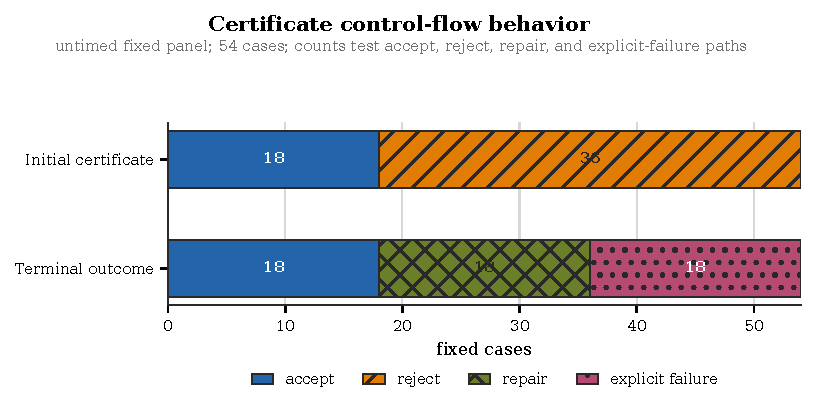
\includegraphics[width=0.82\linewidth]{figures/a42/a42_certificate_behavior.pdf}
\caption{A42 fail-closed behavior.  An initial rejection can lead to a
separately verified repair; domain-invalid inputs produce no allocation.}
\label{fig:behavior}
\end{figure}

A separate sharpness panel uses \AFTwoSharpnessRecords{} fixed candidates across
three graph families, three scales, and seven perturbation radii.  Exact
high-precision replay finds all \AFTwoSharpnessRecords{} recovered allocations
positive, and the edgewise signed predicate proves positivity in all
\AFTwoSharpnessRecords{} cases; the global $\ell_1$ screen proves only 158.
Across relative tolerances $10^{-6},\ldots,10^{-14}$, neither predicate has a
false accept.  Whenever the exact recovery gap is below a tested tolerance, the
production signed predicate also accepts, giving 100\% recall on the applicable
fixed-candidate cells.  At tolerance $10^{-10}$ alone, the edgewise predicate
authorizes \AFTwoSharpEdgeOnlyAtTen{} candidates rejected by the global screen.

The median signed IEEE bound divided by the exact recovery gap is
$1.00000072$, whereas the median global-screen inflation is
\texttt{\AFTwoGlobalInflationMedian}.  The exact-real structural bound has
median inflation $1.00000097$, and its nonzero-radius excess has log--log slope
$0.9883$ as the perturbation shrinks.  Signed cancellation does not change the
accept/reject count on this grid, but it can reduce the same-enclosure
absolute-correction bound to 0.112 of its value.  Zero-radius cells expose an
unavoidable floating-point enclosure floor and are reported separately in the
artifact.  These observations support the fixed-candidate sharpness mechanism
in \cref{prop:asymptotic-completeness}; they do not establish completeness
for arbitrary binary64 candidates.

\begin{figure}[t]
\centering
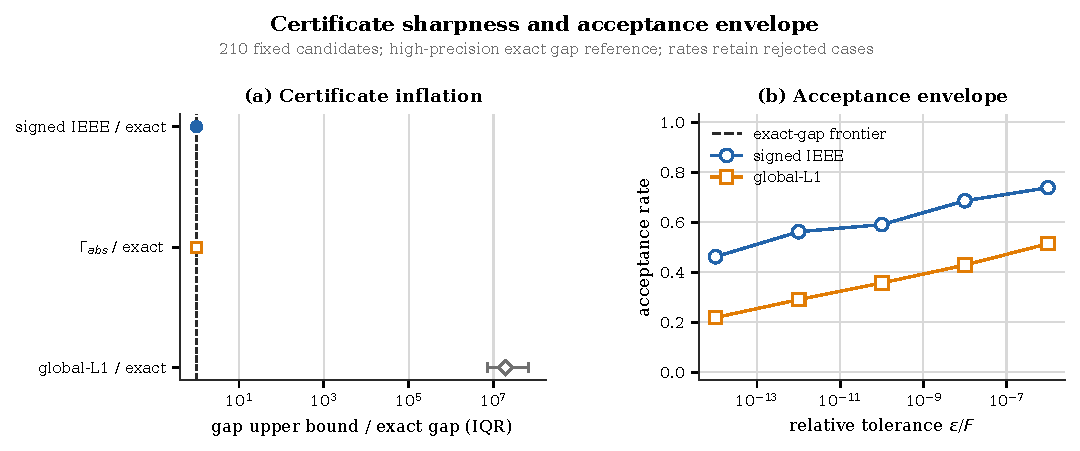
\includegraphics[width=\linewidth]{figures/a42/a42_certificate_sharpness.pdf}
\caption{Certificate sharpness against high-precision exact-recovery
quantities.  The edgewise signed construction retains local correction
information that the global $\ell_1$ screen discards.}
\label{fig:sharpness}
\end{figure}

\subsection{Linear data structures, verifier scaling, and complete-pipeline scaling}
\label{sec:results-scaling}

The exact $m-g$ addition count matters on highly irregular incidence arrays.
We therefore stress the grouped-reduction compiler with one giant group and
many singleton groups at sizes from 30,000 to ten million.  All
\AFTwoSkewRecords{} cells satisfy the node-count, workspace, storage,
execution, and enclosure checks.  The 30 cells through 300,000 inputs also
bitwise-match the independently executed levelwise reference; larger cells use
the registered analytic/high-precision enclosure.  The plan uses 10 index
bytes per input, below its 12-byte registered bound, and the descriptive time
slope is \AFTwoSkewSlope.  In particular, completed singleton groups leave the
active frontier instead of being carried through later levels
(\cref{fig:skewed-reduction}).

\begin{figure}[t]
\centering
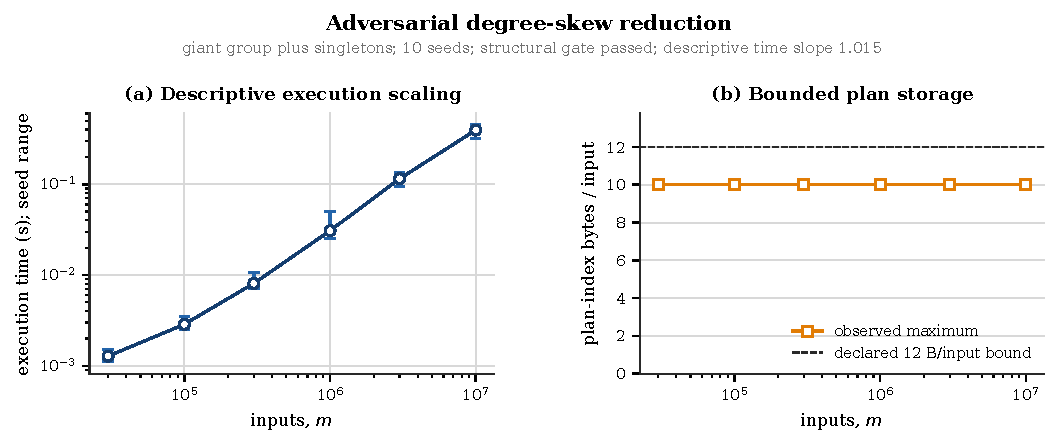
\includegraphics[width=\linewidth]{figures/a42/a42_skewed_reduction.pdf}
\caption{Adversarial segmented-reduction stress.  Exact plan storage stays
linear under the one-giant-group-plus-singletons degree pattern.}
\label{fig:skewed-reduction}
\end{figure}

Verifier-only scaling contains 60 graph--seed cells and 180 timed replays.
The seed-clustered exponent is \AFTwoVerifierSlope{} (95\% interval
$[\AFTwoVerifierSlopeLow,\AFTwoVerifierSlopeHigh]$).  The interval excludes
one, so we describe the measurement as near-linear rather than claiming an
exact empirical exponent.  The largest instance has
\AFTwoVerifierLargestEdges{} edges, a geometric-mean replay time of 3.182
seconds, and \AFTwoVerifierLargestBytesPerEdge{} measured topology-plan bytes
per edge.  Cold problem- and tree-plan construction is recorded but excluded
from this verifier-only timing.

\begin{figure}[t]
\centering
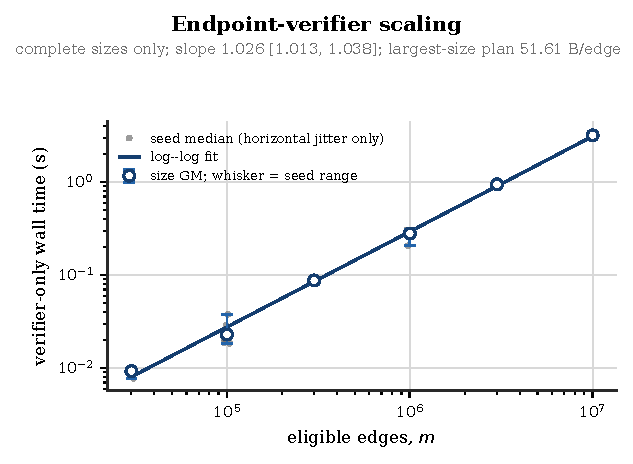
\includegraphics[width=\linewidth]{figures/a42/a42_verifier_scaling.pdf}
\caption{Verifier-only scaling through ten million edges.  Points are
graph-seed medians; the fitted interval clusters by seed.}
\label{fig:scaling}
\end{figure}

The complete pipeline adds candidate generation, strict-state preparation, endpoint
verification, fallback accounting, and materialization.  It contains
\AFTwoPipelineRecords{} records: 45 setup/warmup cells and
\AFTwoPipelineMeasurements{} timed measurements across three graph families.
Every timed measurement returns a strict endpoint.  \Cref{tab:pipeline-scaling}
shows the graph-family--seed median geometric means.  At three million edges
the complete time is \AFTwoPipelineLargestGMSeconds{} seconds.  Its descriptive
slope, \AFTwoPipelineSlope, is higher than the verifier-only slope; candidate
generation consumes a mean fraction \AFTwoPipelineCandidateShare{} of wall
time, versus \AFTwoPipelineVerifyShare{} for verification.  This phase profile
is consistent with, but does not by itself explain, the slope difference.  The
pipeline slope was explicitly not a publication gate.  Here ``complete'' means
the public \texttt{solve\_verified} call through returned materialization after
cold graph, router, and topology-plan setup; it is not first-use end-to-end
latency.

\begin{table}[t]
\centering
\caption{A42 complete solve--verify--materialize scaling.  Each size aggregates
nine graph-family--seed medians; all \AFTwoPipelineTimedAccepts{} timed
measurements are endpoint-accepted.}
\label{tab:pipeline-scaling}
\small
\begin{tabular}{rr}
\toprule
Edges & GM complete-pipeline seconds \\
\midrule
30,000 & 0.06005 \\
100,000 & 0.15190 \\
300,000 & 0.92186 \\
1,000,000 & 3.05713 \\
3,000,000 & \AFTwoPipelineLargestGMSeconds \\
\bottomrule
\end{tabular}
\end{table}

Together, the skew, verifier-only, and complete-pipeline panels distinguish
three claims that are often conflated: exact linear plan size, near-linear
observed verifier time, and the larger cost of whatever candidate generator is
placed in front of the verifier.

\subsection{Dynamic and strict-pipeline cost}
\label{sec:results-dynamic}

The dynamic panel evaluates 1,050 paired rounds at 100,000 edges.  CertQuota-V
returns a strict, matched endpoint on every round with geometric-mean complete
time \AFTwoDynamicVGMSeconds{} seconds.  The interval-screened stepwise strict
pipeline takes 0.362664 seconds, so the paired V/stepwise ratio is
\AFTwoDynamicVOverStepwise{} (95\% interval $[0.28449,0.29793]$).
Uncertified damped Newton is faster at
\AFTwoDynamicDampedGMSeconds{} seconds: V/damped is
\AFTwoDynamicVOverDamped{} (95\% interval $[1.4354,1.4884]$).
The latter returns numerically matched points but supplies no strict endpoint
authority, and is therefore an overhead reference rather than a certified
competitor.

\begin{figure}[t]
\centering
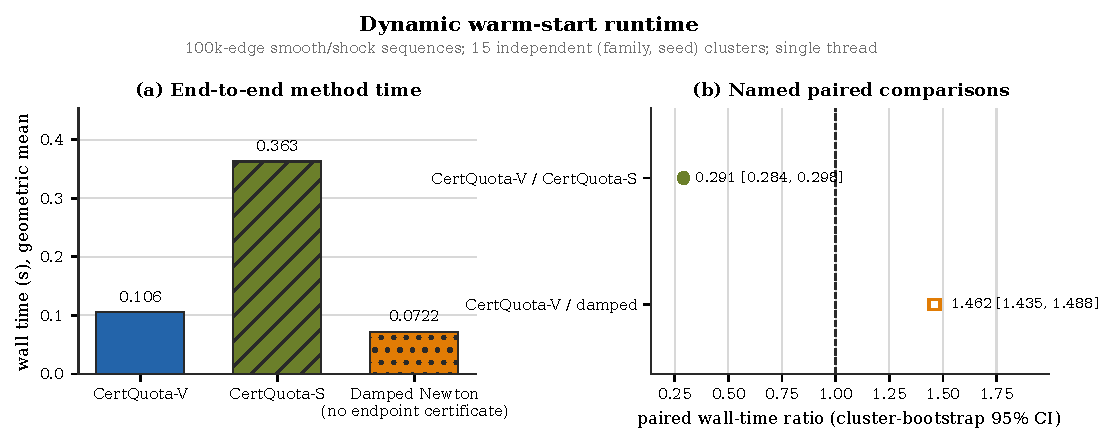
\includegraphics[width=\linewidth]{figures/a42/a42_dynamic_runtime.pdf}
\caption{Complete dynamic time and paired ratios.  The dashed line marks equal
time; damped Newton is deliberately shown as an uncertified numerical
reference.}
\label{fig:dynamic}
\end{figure}

The warm-start basin screen passes only \AFTwoBasinPasses{} of
\AFTwoBasinRounds{} rounds: all 300 smooth $10^{-3}$ updates and 420 non-jump
shock-sequence rounds, but neither the 300 smooth $10^{-2}$ updates nor the 30
shock jumps.  Nevertheless, the final endpoint verifier accepts
\AFTwoEndpointAccepts{}/\AFTwoDynamicRounds{} CertQuota-V outputs.  Thus basin
membership is a useful local diagnostic, not the authority for the returned
allocation; the solve--verify cascade can recover outside that diagnostic
region.

All four named strict pipelines also certify and match each of 75 frozen
100,000-edge rounds.  \Cref{tab:strict-pipelines} reports their descriptive
cost.  CertQuota-V is the lowest-time implementation in this panel, but the
other three reuse portions of our recovery or certification machinery, so the
panel cannot support a general fastest-solver claim.  Alternate scaling is
especially long-tailed: its median is
\AFTwoStrictScalingMedianSeconds{} seconds, while its 90th and 95th percentiles
are \AFTwoStrictScalingPninetySeconds{} and
\AFTwoStrictScalingPninetyfiveSeconds{} seconds and its maximum is
\AFTwoStrictScalingMaxSeconds{} seconds.

\begin{table}[t]
\centering
\caption{Named strict pipelines at 100,000 edges.  Ratios are paired method
time divided by CertQuota-V time.}
\label{tab:strict-pipelines}
\small
\begin{tabular}{lrr}
\toprule
Strict pipeline & GM seconds & Method/V \\
\midrule
CertQuota-V & 0.110055 & 1.000 \\
Stepwise interval screen & 0.400204 & 3.636 \\
Alternate-scaling verified & \AFTwoStrictScalingGMSeconds & \AFTwoStrictScalingOverV \\
Arb terminal replay & 2.34512 & 21.309 \\
\bottomrule
\end{tabular}
\end{table}

\begin{figure}[t]
\centering
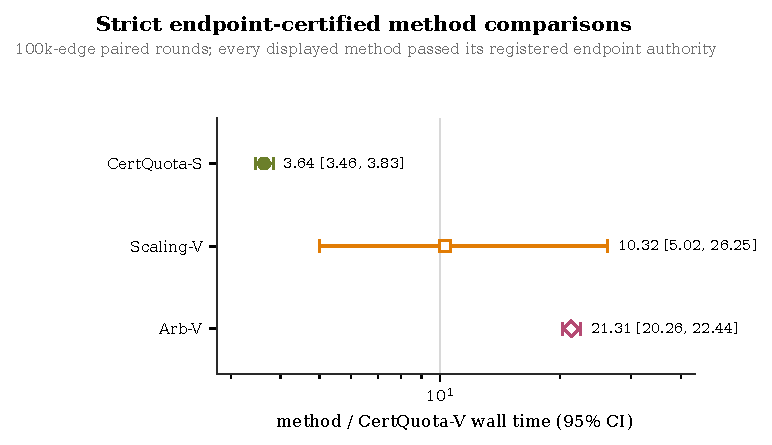
\includegraphics[width=\linewidth]{figures/a42/a42_strict_comparisons.pdf}
\caption{Descriptive ratios for the four named strict pipelines.  Their shared
components limit the comparison to these executed implementations.}
\label{fig:strict-comparisons}
\end{figure}

The conic experiments supply a more independent candidate source.  On 45
small/medium internal cells, both CertQuota-V and Clarabel/CVXPY candidates
receive endpoint certificates.  On the 18-cell external stress grid,
CertQuota-V certifies 18/18, whereas Clarabel reports an optimal candidate on
every cell but only 14/18 pass endpoint replay.  Consequently no strict
external timing ratio is reported.  A standalone Arb implementation, sharing
neither the production interval code nor tree router, reproduces all
\AFTwoIndependentReplays{} decisions at 256 bits and the four rejections again
at 384 bits.  In the rejected cells, its same-dual gap intervals lie wholly
above the respective targets: lower endpoints
$0.0532577,0.0499891,0.0382662,0.0302070$ versus targets
$0.0254701,0.0262432,0.0262347,0.0256089$.  The production upper bounds exceed
the independent values by at most $9.19\times10^{-8}$ percent.  Arb therefore
diagnoses insufficient accuracy of the submitted dual witnesses, rather than
rounding conservatism in the production certificate.  Recovered primals do
pass against the planted reference dual, so the diagnosis does not imply that
the raw primal coordinates are themselves unusable.

\subsection{Materialized conditional-MSE case studies}
\label{sec:results-mse}

The synthetic sampling panel contains 3,200 quota-matched analytic records per
policy and 32,000 nonuniform solves.  All 32,000 emitted probability vectors
have strict endpoint certificates; 20 attempted candidates are rejected and
10 records are repaired by a later cascade stage.  The maximum certified
objective-gap upper bound is $1.07\times10^{-12}$ and the maximum measured
normalized marginal residual after binary64 materialization is
$9.24\times10^{-13}$.  The registered row targets obey
$\max_i r_i\le0.2$; together with this residual bound, every materialized row
mass remains strictly below one.  The analytic MSE uses that same positive
finite vector both as the categorical inclusion law and as the
Horvitz--Thompson denominator.  The current-norm and age-one policies pass the two
registered Holm-adjusted one-sided tests ($p_{\mathrm{adj}}=2.00\times10^{-4}$).

The aggregate effect requires quota stratification
(\cref{tab:mse-by-quota}).  With quota ratio one, the current oracle improves
over quota-matched uniform sampling by only about 0.34\%; at ratio ten, the
improvement is about 14.5\%.  An age-one proxy closely tracks the oracle in
both regimes, while age 20 loses some benefit.  The coordinate proxy is harmful
in both regimes.  Thus the overall oracle ratio
\AFTwoEstimatorOracleMSE{} is not a quota-invariant effect.

\begin{table}[t]
\centering
\caption{Conditional MSE divided by quota-matched uniform MSE at materialized
binary64 probabilities.  The all-cells column is the fixed-grid geometric
mean.}
\label{tab:mse-by-quota}
\small
\begin{tabular}{lrrr}
\toprule
Policy & All cells & Quota ratio 1 & Quota ratio 10 \\
\midrule
Current-norm oracle
 & \AFTwoEstimatorOracleMSE
 & \AFTwoQuotaOneOracleMSE
 & \AFTwoQuotaTenOracleMSE \\
Historical norm, age 1
 & \AFTwoEstimatorStaleOneMSE
 & \AFTwoQuotaOneStaleOneMSE
 & \AFTwoQuotaTenStaleOneMSE \\
Historical norm, age 20
 & \AFTwoEstimatorStaleTwentyMSE
 & \AFTwoQuotaOneStaleTwentyMSE
 & \AFTwoQuotaTenStaleTwentyMSE \\
Coordinate proxy
 & \AFTwoEstimatorCoordinateMSE
 & \AFTwoQuotaOneCoordinateMSE
 & \AFTwoQuotaTenCoordinateMSE \\
\bottomrule
\end{tabular}
\end{table}

\begin{figure}[t]
\centering
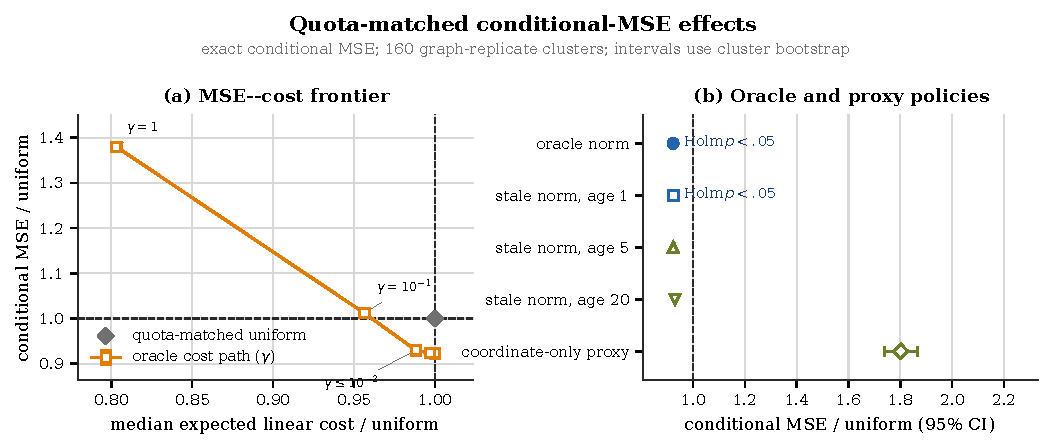
\includegraphics[width=\linewidth]{figures/a42/a42_estimator_effects.pdf}
\caption{Synthetic quota-matched conditional-MSE ratios.  Confidence intervals
cluster by independent graph/update replicate; the dashed line is uniform
sampling.}
\label{fig:estimator-effects}
\end{figure}

MovieLens-1M contributes two deliberately limited forms of non-synthetic
structure.  First, its \AFTwoMovieLensEdges{} observed user--movie interactions
form a connected support with 6,040 users and 3,706 rated movies.  All
\AFTwoMovieLensStrictAccepts{} planted numerical stress instances on that
support certify, closing the synthetic-topology gap but making no recommender
effect claim.

Second, the user--genre panel retrospectively retains the common support having
observations on both sides of each cutoff, then derives positive two-coordinate
update proxies from historical and later temporal rating summaries.  Five temporal cutoffs,
two expected-quota regimes, and three policies give 30 strict endpoints and
\AFTwoGenreCells{} paired cells.  The current-weight oracle has overall
conditional-MSE ratio \AFTwoGenreOracleOverEqual{} against equal edge weights;
the historical proxy has ratio \AFTwoGenreHistoricalOverEqual{} against equal
and \AFTwoGenreHistoricalOverOracle{} against the current oracle.  Under equal
model quotas, the current/equal and historical/equal ratios are
\AFTwoGenreEqualOracleOverEqual{} and 0.973635; under popularity-aware quotas
they are \AFTwoGenrePopularityOracleOverEqual{} and 1.02778.  The historical
proxy therefore helps relative to equal weights only in the equal-quota
regime, while current weights help in both
(\cref{fig:movielens-genre}).

\begin{figure}[t]
\centering
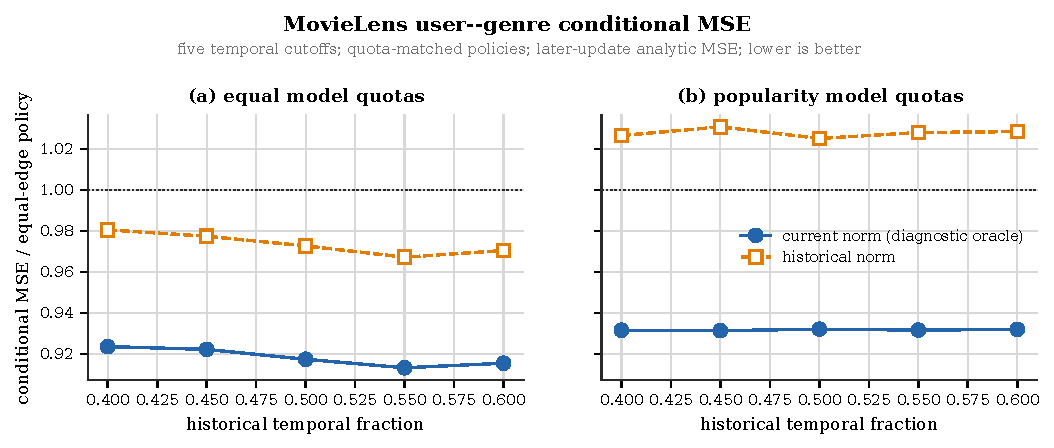
\includegraphics[width=\linewidth]{figures/a42/a42_movielens_genre_sampling.pdf}
\caption{MovieLens user--genre conditional-MSE ratios over five temporal
cutoffs on retrospectively selected common support.  This is a descriptive
allocation study: it does not train a neural model or evaluate recommendation
accuracy.}
\label{fig:movielens-genre}
\end{figure}

The two case studies establish that certified reciprocal allocations can be
materialized and evaluated on both controlled update fields and a public sparse
interaction structure.  They do not establish federated-learning accuracy,
training-time, or recommender-system state of the art.

\subsection{Tree sensitivity and a historical-only public workload}
\label{sec:results-a43}

The disjoint A43 amendment first holds each candidate fixed and changes only
the spanning tree.  Its 36 graph--candidate pairs cross three graph families,
two scales, three seeds, and two registered perturbation radii; four tolerances
and four preregistered tree rules produce \AFThreeTreeRecords{} strict replays.
Every replay proves positivity, so tree choice does not alter the soundness
theorem.  It does materially alter sharpness: \AFThreeTreeDisagreements{} of
\AFThreeTreeCells{} candidate--tolerance cells have different acceptance
decisions across trees.  The median and 95th-percentile within-cell ratios of
largest to smallest finite gap bound are \AFThreeTreeGapRatioMedian{} and
\AFThreeTreeGapRatioPninetyfive{}.  The registered tree-insensitivity gate
therefore fails by a wide margin.

\begin{table}[t]
\centering
\caption{A43 spanning-tree sensitivity on identical candidates.  Positivity
is certified in all 144 replays for every rule; acceptance additionally
requires the registered objective tolerance.  The last column is the median
maximum tree-edge correction divided by the uncorrected allocation.}
\label{tab:tree-sensitivity}
\small
\begin{tabular}{lrrr}
\toprule
Tree rule & Accepted & Positive & Median relative correction \\
\midrule
Input order & \AFThreeTreeInputAccepts/144 & 144/144
 & \AFThreeTreeInputCorrectionMedian \\
Maximum conductance & \AFThreeTreeMaxConductanceAccepts/144 & 144/144
 & \AFThreeTreeMaxConductanceCorrectionMedian \\
Minimum conductance & \AFThreeTreeMinConductanceAccepts/144 & 144/144
 & \AFThreeTreeMinConductanceCorrectionMedian \\
Seeded random & \AFThreeTreeRandomAccepts/144 & 144/144
 & \AFThreeTreeRandomCorrectionMedian \\
\bottomrule
\end{tabular}
\end{table}

Maximum-conductance Kruskal is never rejected in a cell where another rule is
accepted.  It accepts all 36 candidates at each of relative tolerances
$10^{-10}$, $10^{-8}$, and $10^{-6}$, and 18 of 36 at $10^{-12}$, for
\AFThreeTreeMaxConductanceAccepts{}/144 overall.  This is an empirical selection
rule, not a theorem that it minimizes the certificate bound.  For new
workloads we therefore recommend selecting a maximum-conductance tree from the
candidate state, then compiling and freezing that tree before endpoint replay.
Its construction cost is outside the fixed-topology linear-work claim and must
be reported separately.

The second A43 panel removes future-dependent support selection.  At each
cutoff it reads only historical MovieLens rows, retains user--genre pairs with
at least two historical ratings in the largest connected component, derives
$\mu$ from two historical rating coordinates, and induces both marginal
families from historical pair counts.  It starts from the public
\texttt{dual\_feasible\_start}; no planted optimum or future potential enters
the problem.  All \AFThreeMovieAccepts{} workloads receive an endpoint
certificate on their first damped-Newton attempt (\cref{tab:historical-workload}).

\begin{table}[t]
\centering
\caption{A43 MovieLens workload using ratings at or before each cutoff only.
All instances have 18 active genres.  Times are single registered-machine
observations and are descriptive, not a scaling comparison.}
\label{tab:historical-workload}
\small
\begin{tabular}{rrrrrr}
\toprule
Cutoff & Users & Edges & Gap upper bound & $\ell_1$ residual & Seconds \\
\midrule
0.40 & \AFThreeMovieUsersA & \AFThreeMovieEdgesA
 & \AFThreeMovieGapA & \AFThreeMovieResidualA & \AFThreeMovieSecondsA \\
0.50 & \AFThreeMovieUsersB & \AFThreeMovieEdgesB
 & \AFThreeMovieGapB & \AFThreeMovieResidualB & \AFThreeMovieSecondsB \\
0.60 & \AFThreeMovieUsersC & \AFThreeMovieEdgesC
 & \AFThreeMovieGapC & \AFThreeMovieResidualC & \AFThreeMovieSecondsC \\
\bottomrule
\end{tabular}
\end{table}

The first accepted result is also exported as exact binary64 arrays, candidate,
tree, tolerance, and a canonical SHA-256 payload.  A fresh reconstruction reruns
the strict backend, accepts, and exactly matches the serialized claim
fingerprints.  This closes the process-local usability gap without turning the
JSON summary into authority.  The panel establishes a public, historical-input
optimization workload and portable endpoint replay; it does not evaluate
recommendation accuracy or causal deployment performance.

\subsection{Experimental external verified-conic baseline}
\label{sec:results-a44}

The disjoint A44 amendment executes VSDP 2020.1 as the closest identified
general verified-conic comparator on small and medium instances.
Each reciprocal term is represented by one three-dimensional
second-order cone and five lifted variables; power-of-two scaling keeps the
transformation exact for the represented binary64 coefficients.

The VSDP and SeDuMi sources are pinned upstream releases.  A thin adapter maps
VSDP's SOCP uses of INTLAB onto the GNU Octave interval package.  This is an
experimental open-backend port, not INTLAB and not an official stock-VSDP
configuration.  Before the confirmatory run, it passed a sub-ulp outward
interval-construction test, a verified linear-solve containment test, and the
VSDP authors' bundled SOCP rigorous-bound assertions.

All 18 preregistered cells cross three graph families, two edge counts, and
three seeds. Their complete represented-problem fingerprints match the
corresponding immutable A42 CertQuota cells. The experimental port reported
finite lower and upper objective bounds in 18/18 cells. Every bracket
contained the floating planted reference objective, used only by the analysis.
This reference is not an exact optimality witness for the represented input:
rounding the constructed flow, costs, and marginals generally breaks exact
KKT equalities. Reference containment is consequently a consistency diagnostic,
not a correctness test. Moreover, all 18 A44 interval widths exceed the paired
A42 requested tolerances (by factors 10.23--121.03); finite-bracket success
must not be read as matched-accuracy success.
\Cref{tab:vsdp-port-a44} reports interval width and resource use.  The two
methods have different process and runtime boundaries, so this amendment
does not authorize a direct speed ratio.

\begin{table}[t]
\centering
\caption{A44 experimental VSDP 2020.1/GNU Octave interval-port results on
the 18 source-bound confirmatory cells.  Each size contains three graph
families and three seeds.  Time is a fresh Octave process per cell and RSS is
the observed process-tree peak; neither is directly comparable with the
historical in-process A42 timings.}
\label{tab:vsdp-port-a44}
\small
\begin{tabular}{rrrrr}
\toprule
Edges & Rigorous brackets & Median relative width & Median seconds & Median MiB \\
\midrule
300  & 9/9 & $2.02\times10^{-8}$ & 4.98 & 219 \\
1000 & 9/9 & $7.07\times10^{-8}$ & 29.45 & 1705 \\
\bottomrule
\end{tabular}
\end{table}


Thus A44 supplies an executed general conic rigorous-bound path and removes
the earlier absence of any such run at the algorithm level.  It does not close
the narrower stock VSDP+INTLAB comparison: a licensed INTLAB installation was
not available, and the experimental rows remain ineligible for an official or
direct speed-ranking claim.

\subsection{Independently witnessed, matched-accuracy revision}
\label{sec:results-a45}

A45 is an exploratory response to the preceding limitations, not a new
preregistered confirmation of the already inspected A44 instances. A disjoint
120-edge pilot (seed 45001, three families) tests SeDuMi tolerances
$10^{-10},10^{-12},10^{-14}$ and retains all nine attempts. Matched, independently
proved brackets occur in respectively 0/3, 3/3 and 2/3 cases, selecting
$10^{-12}$ before the 18-instance rerun. The new runs use exactly the paired
A42 problem fingerprints and requested $\varepsilon$ values, not an optimizer
status or a floating planted objective as ground truth.

\paragraph{Independent witnesses.}
A standard-library-only checker uses integer-directed dyadic arithmetic at
160 fractional bits. For endpoint bundles it directly encloses $P(Z)$ and
$D(y)$, without the production interval backend or its cancellation identity.
For each experimental VSDP-port bracket, it reconstructs the lifted dual
inequalities from the original data, verifies the LP and squared Lorentz-cone
conditions in exact rational arithmetic, and checks the correctly rescaled
conic dual objective against $L$. Separately,
exact rational leaf elimination of an exported primal midpoint supplies a
positive feasible original flow whose outward objective bound is at most $U$.
Thus the saved witnesses prove that particular original-input bracket even
without trusting the port's interval linear solve. They do not validate every
operation of the compatibility layer or establish a stock INTLAB result.
Additional tests use ten genuinely exact dyadic KKT fixtures and 252 exact
right-hand-side corner solves across 12 small linear systems; floating planted
reference containment is never used as a correctness gate.

\paragraph{Common accuracy and cost boundaries.}
Both pipelines run in fresh single-thread processes under 300-second and
4096-MiB sampled-RSS limits. Common MAT export is excluded; the port's external
dyadic lift construction is charged separately. Verification time includes
VSDP's internal perturbed re-solves, or CertQuota's cold tree/plan preparation
and replay. The transfer test uses the same initial SeDuMi dual, without a
CertQuota repair. Full pipeline time adds process startup and an independent
witness-check process; these audited pipelines are distinct from warm replay
throughput. Peak RSS below concerns the numerical worker, not the separate
integer audit. Timings describe these implementations on the recorded host.

\begin{table}[t]
\centering\small
\caption{A45 first-setting comparison; times are medians over all nine cells
at each size, including accuracy failures. Port denotes only the experimental
VSDP/Octave-interval implementation, whose linear-solve path densifies.
CQ-transfer certifies all 18 initial SeDuMi duals; the full CQ column uses its
own public cold candidate pipeline. These are not stock-VSDP speed estimates.}
\label{tab:a45-matched}
\setlength{\tabcolsep}{3pt}
\begin{tabular}{rrrrrrr}
\toprule
$m$ & \multicolumn{2}{c}{Matched / 9} &
\multicolumn{2}{c}{Verification (s)} & \multicolumn{2}{c}{Audited pipeline (s)}\\
 & Port & CQ & Port & CQ-transfer & Port & CQ\\
\midrule
300 & \AFiveSmallPortPass & 9 & \AFiveSmallPortVerify & \AFiveSmallTransferVerify & \AFiveSmallPortPipeline & \AFiveSmallCQPipeline\\
1000 & \AFiveMediumPortPass & 9 & \AFiveMediumPortVerify & \AFiveMediumTransferVerify & \AFiveMediumPortPipeline & \AFiveMediumCQPipeline\\
\bottomrule
\end{tabular}
\end{table}

All 18 port brackets have independently checked witnesses;
\AFivePortMatched/18 meet the common target, whereas both CertQuota's full
pipeline and the unrepaired SeDuMi-dual transfer meet it in 18/18 cases.
The remaining three port widths are 1.77--2.22 times their targets. A fixed
second setting, $10^{-14}$, is tried for every first-setting failure, charging
both attempts to the same time budget; it adds no matched success. All attempts
are retained. This is not a lower bound on the accuracy obtainable by VSDP after
other tuning. At 1000 edges, median worker RSS is
\AFiveMediumPortRSS\ MiB for the port and \AFiveMediumCQRSS\ MiB for CertQuota;
the dense compatibility path prevents attributing that difference to stock
VSDP. The defensible computational conclusion is narrower: on these identical
inputs, an original-array endpoint check accepts the same approximate duals
with substantially less measured verification work than this executed conic
path, at the stated common guarantee.

\subsection{A historical decision workload with an explicit rational output}
\label{sec:a45-decision}

The revision uses three additional MovieLens history cutoffs
$(0.45,0.55,0.65)$. Every support edge, reciprocal weight and processing proxy
uses only pre-cutoff records. Client budgets are fixed to the represented value
0.2. Genre quotas are specified before optimization as
$(1-\theta)d^{\rm hist}+\theta(0.2n_{\rm left}/n_{\rm genre})\one$, with
$\theta\in\{0,0.25\}$ and the same exact reduced-root convention. Historical
rating counts $k_e$ define nonzero costs $c_e=\lambda k_e$; $\lambda$ is
normalized so that baseline processing cost is approximately $0.1$ or $1$
times baseline reciprocal cost. These are explicit task-design proxies, not
measured production latencies. Raking supplies an approximate baseline, which
is repaired and checked as an exactly feasible rational flow before it is
used for the policy comparison.

Let $[L_0,U_0]$ enclose that feasible baseline's objective. The pre-specified
decision asks whether a feasible allocation can meet the cap $0.99L_0$;
the requested gap is $10^{-8}(1+U_0)$. A rational allocation $\widehat Z$
is exported with all numerators and denominators, rather than claimed to be
bitwise feasible in binary64. Its independent checker tests $B\widehat
Z=\beta$ exactly, strict positivity, and an objective interval. It returns
``below cap'', ``cap infeasible'', or ``undecided'' according to the proved
upper and lower endpoints, never a rounded point estimate. All
\AFiveWorkloadAccepted/12 combinations certify, and all prove at least the
requested 1\% improvement over their own feasible baseline. The conservative
improvement bounds range approximately from \AFiveImprovementMin\% to
\AFiveImprovementMax\%. This demonstrates a usable mathematical policy
decision and a transferable exact allocation; it does not establish a
statistical improvement in a deployed recommender or MMFL training system.
The 12 combinations share one dataset, not 12 independent applications.

\subsection{Hard starts and dynamic tree rebuilding}
\label{sec:a45-hard}

Nine new family--seed graphs (seeds 45101--45103) discard the generator's
KKT-planted costs and replace them by independently drawn positive costs.
Two reciprocal-weight spans, quota shocks, public cold starts and candidates
within $10^{-10}$ relative slack of the dual-domain boundary give 36 valid
hard-start cases (18 represented problems, two starts per problem). CertQuota
independently certifies \AFiveColdAccepted/18 public cold starts and
\AFiveBoundaryAccepted/18 near-boundary starts under a 20-second budget.
All 18 deliberately out-of-domain controls are rejected. Failed candidates
and repairs are retained separately from accepted endpoints; these tests do
not replace the earlier warm-start scalability study.
All ten valid failures receive an explicit optional follow-up: a
CVXPY/Clarabel candidate with a 10-second budget followed by up to 10 seconds
of the unchanged strict pipeline. Seven certify. The remaining three conic
duals, despite an approximate optimal status, lie outside the original dual
domain; convex retraction toward a public domain point and another bounded
refinement certify all three. Thus 36/36 valid starting cases eventually have
independently checked endpoints, while the original 26/36 result and all
additional work remain visible. This is an exploratory repair study with extra
budget, not a claim that the unchanged 20-second default succeeds universally.

The same held-out family--seed grid then exercises eight changing rounds and
three tolerances. Three explicit policies keep the initial maximum-conductance
tree, rebuild it every round, or rebuild only after a failed replay. Each
policy has 216 candidate--tolerance cells. Construction, cold router plans,
preparation and retries are charged, policy order rotates, and candidate
generation is recorded separately. Multiple rounds and tolerances are not
independent graph samples.
\begin{table}[t]
\centering\small
\caption{Held-out A45 dynamic-policy comparison. Times include unsuccessful
checks and rebuilds but exclude the common candidate generator. These are
finite policy observations, not a universal optimal-tree guarantee.}
\label{tab:a45-trees}
\begin{tabular}{lrrr}
\toprule
Policy & Accepted / 216 & Tree builds & Total policy time (s)\\
\midrule
Frozen tree & \AFiveFrozenAccepted & \AFiveFrozenBuilds & \AFiveFrozenSeconds\\
Rebuild every round & \AFiveAlwaysAccepted & \AFiveAlwaysBuilds & \AFiveAlwaysSeconds\\
Rebuild after rejection & \AFiveRetryAccepted & \AFiveRetryBuilds & \AFiveRetrySeconds\\
\bottomrule
\end{tabular}
\end{table}
The production default was already maximum conductance before this revision;
the new evidence concerns when to reuse or rebuild, not the discovery of that
default. Rejection-triggered rebuilding remains a measured policy with an
explicit extra cost, not part of the fixed-topology complexity theorem.
On this grid it matches the always-rebuild acceptance count using 66 rather
than 216 builds, with 1.112 rather than 1.943 seconds total policy cost. The
frozen policy is cheaper but rejects 38 cells. This makes the reuse--rebuild
tradeoff explicit; no tree is asserted to be uniformly best.


\section{Related work}
\label{sec:related}

\paragraph{Reciprocal transport and convex network flow.}
The objective itself is not new.  The $\beta$-potential formula of
Dessein et al.\ \citep{dessein2018rot}, extended algebraically beyond its analyzed parameter
range, gives
\[
 \phi_{-1}(z)=\frac{z^{-1}+z-2}{2},\qquad
 c_ez_e+\frac{\mu_e}{z_e}
 =(c_e-\mu_e)z_e+2\mu_e\phi_{-1}(z_e)+2\mu_e.
\]
Thus our weighted objective is a formal edge-weighted $\beta=-1$
specialization after an edgewise shift of the linear costs and an additive
constant.  This is an algebraic identification, not an inherited algorithmic
guarantee: Dessein et al.\ \citep{dessein2018rot} analyze $0<\beta<1$ for this family and
explicitly note that other parameter values need not satisfy their assumptions.
Newton and interior methods for separable nonlinear network and transportation
 problems are classical
 \citep{klincewicz1983,klincewicz1989,katsura1989interior,ibaraki1991dual}.
 Earlier primal algorithms already maintain feasible convex-cost flows and
 derive objective upper bounds: the method in \citep{weintraub1974primal} uses the most
 negative incremental-cost circuit both to update a feasible flow and to bound
 its remaining suboptimality.  The $\epsilon$-relaxation method of
 \citep{bertsekas1997epsilon} is globally terminating and near-optimal
 with a complexity analysis.  These are solver algorithms with their own
 iterates and termination logic, rather than posterior outward-rounded replay
 contracts for arbitrary candidate arrays.

 Primal recovery from a nonoptimal dual vector is also not new:
 \citep{marklund2008early} constructs primal-feasible flows for separable
 strictly convex single-commodity networks using residual-graph and
 shortest-path schemes, with convergence to the unique primal optimum along a
 convergent dual sequence and an associated primal--dual stopping criterion.
 Their construction is therefore also usable around dual algorithms rather
 than tied to one candidate generator.  Its real-arithmetic recovery is not an
 outward-rounded finite endpoint replay, does not require edgewise strict
 positivity, and does not state an original-array $O(m+n)$ certificate bound.
More recent work exploits bipartite normal equations, sparsity, and
regularization at far greater generality
\citep{castro2021huge,wright2023direct,cipolla2024sparse,tang2024safe,
wang2025splr};
almost-linear flow algorithms address broader objectives
\citep{chen2025maxflow}.  Finite-precision primal recovery and explicit gaps
also appear in an almost-linear solver for a different hypergraph-Laplacian
energy \citep{yoshida2026hypergraph}.  We do not claim a new Newton method,
Laplacian Hessian, finite-precision graph recovery, reciprocal formulation, or
globally near-linear candidate solver.
The Convex Network Flows framework covers a broader class of hypergraph flow
models and supplies an edge-decomposed algorithm and the open-source
ConvexFlows.jl implementation \citep{diamandis2024convexflows}.  It is therefore
a relevant general solver and software precedent, but does not make the signed
original-array endpoint claim studied here.
Recent OT candidate solvers combine truncated or sparse Newton steps with
Sinkhorn or Bregman proximal frameworks
\citep{kemertas2025truncated,wu2025pins,pan2026ibsn}; a contemporaneous
network-equilibrium preprint reports empirical near-linear scaling for a
different undirected model \citep{livne2026nlf}.  These works strengthen
candidate generation and global solution, whereas our theorem concerns a
finite, solver-independent endpoint replay on the represented reciprocal
problem.  A recent dynamic-OT Newton method uses a spanning-tree gauge to remove
cycle redundancy and a separate CFL positivity condition
\citep{chen2026graphot}; that use of a tree is distinct from our
support-preserving endpoint residual repair and precludes any claim that trees
or positivity are new to OT Newton methods.

Approximate transport algorithms often postprocess marginals.  The rounding
construction in \citep{altschuler2017nearlinear}, for example, can add a residual
outer product and need not preserve a prescribed sparse eligibility support.
Our spanning-tree correction instead stays on declared edges and couples exact
marginal repair to an explicit strict-positivity and objective-gap test.  That
support-preserving certificate, rather than rounding in general, is the
structure used here.

\paragraph{Verified optimization.}
Separating a fast computation from a checkable witness is the certifying
algorithm paradigm \citep{mcconnell2011certifying}.  Rigorous objective bounds
and postprocessing exist for convex, conic, linear, and semidefinite programs;
general accuracy certificates formalize how computed information can authorize
quantitative error statements
\citep{nemirovski2010accuracy,jansson2009verified,jansson2004convex,
jansson2007conic,jansson2007rigorous,lange2020verification,rump2010verification}.
Interval methods can separately prove equality-constrained feasibility
\citep{kearfott1998feasible}, while modern certificate formats and formally
verified floating-point kernels address proof portability and trusted
implementation boundaries in other problem classes
\citep{szeider2026vipr,kohlen2025verified}.
General conic dual certificates can also reconstruct or certify primal cone
membership, and feasible nonsymmetric conic interior-point methods can produce
compatible near-optimal candidates
\citep{lee2025dual,papp2025fullnewton}; therefore neither posterior
certification nor dual-to-primal reconstruction is new in principle.
Fast feasible primal recovery from dual iterates is also studied beyond network
flow \citep{parshakova2025multiple}, and accelerated primal--dual averaging can
produce general convex accuracy certificates \citep{burns2026accuracy}.
Verified DCP/conic reductions in Lean address the complementary modeling
boundary \citep{bentkamp2023verified}; our artifact does not claim a formally
verified reduction from an application model.  Standard conic quadratic
formulations and primal--dual implementations
\citep{andersen2003conic,goulart2026clarabel,diamond2016cvxpy} apply to
\cref{eq:problem} after introducing one cone block per edge.

VSDP is the closest identified general rigorous software comparator: it can
verify linear, second-order-cone, and semidefinite programs, but its documented
runtime requires MATLAB or GNU Octave, INTLAB, and an approximate conic solver
\citep{vsdp2020}.  None of MATLAB, Octave, or INTLAB was present in the frozen
A42/A43 environment, so stock VSDP was unavailable there rather than encoded
as a synthetic timeout.  A44 subsequently pins VSDP and SeDuMi and executes
the SOCP rigorous-bound routines through an audited experimental GNU Octave
interval adapter.  The adapter result is reported explicitly as an open-backend
port and is not relabeled as stock VSDP+INTLAB.  The executed CVXPY/Clarabel
lift measures candidate transfer, while Arb measures an independent replay of
our predicate; neither is a general verified optimizer.  A44 removes the lack
of an executed generic conic bound computation. A45 adds exact per-instance
witness checks, common tolerances and fresh-process timing. The absent official
INTLAB configuration and the port's dense interval path still prevent a general
performance claim against verified conic software.

Our narrower distinction is the simultaneous contract of an endpoint replay on
the original $(B,\beta,c,\mu)$ arrays: no $m$-block conic lift or generator
status is trusted, tree recovery preserves sparse support, signed outward
intervals prove strict positivity and a gap for the same implicit exact-real
allocation, and the fixed-topology replay has $O(m+n)$ work and memory.  Feasible
primal recovery, objective-gap bounds, interval verification, trees, and fast
convex-flow software all have prior art; the contribution is their
structure-specific combination in one finite endpoint decision procedure.
Arb-V is a separately implemented higher-precision audit of the same endpoint predicate
\citep{johansson2017arb}; it is neither an external method nor evidence that
general verified conic software is inferior.

\Cref{tab:novelty-map} separates capabilities already present in prior work
from their combination in our endpoint predicate.  Entries marked
\emph{no endpoint claim} are outside the cited method's stated output contract;
they do not assert impossibility within that broader framework.
% Compact MPC-layout capability map.
\begin{table}[t]
\centering
\caption{Relation to the closest method families.  ``No finite endpoint'' means
that the cited work does not state the simultaneous outward-rounded guarantee
in the third column; it is not an impossibility claim.}
\label{tab:novelty-map}
\scriptsize
\setlength{\tabcolsep}{3pt}
\renewcommand{\arraystretch}{1.12}
\begin{tabular}{@{}
>{\raggedright\arraybackslash}p{0.20\linewidth}
>{\raggedright\arraybackslash}p{0.23\linewidth}
>{\raggedright\arraybackslash}p{0.27\linewidth}
>{\raggedright\arraybackslash}p{0.23\linewidth}@{}}
\toprule
Method family & Native object & Finite endpoint contract & Distinction here \\
\midrule
Reciprocal transport and classical convex network flow
\citep{dessein2018rot,weintraub1974primal,klincewicz1983,
klincewicz1989,bertsekas1997epsilon,marklund2008early}
& Transport or network arcs; support is native
& Feasible iterates, recovery, and stopping bounds in real arithmetic; no
single outward-rounded arbitrary-candidate endpoint
& Same sparse support, but one finite replay binds positivity, exact-real
feasibility, and the gap \\

General convex-flow solvers
\citep{chen2025maxflow,diamandis2024convexflows}
& Graph or hypergraph flow model
& Solver-dependent global guarantees; no arbitrary-candidate endpoint replay
& Original reciprocal arrays and generator-independent return authority \\

Transport rounding \citep{altschuler2017nearlinear}
& Dense transport plan
& Exact-arithmetic marginal repair; strict positivity and endpoint gap are not
the target
& Tree repair remains on the declared sparse support \\

Verified conic and interval optimization
\citep{jansson2004convex,jansson2007conic,jansson2007rigorous,
jansson2009verified,lange2020verification,vsdp2020,rump2010verification}
& Generic lifted cone or nonlinear/KKT enclosure
& Rigorous formulation-dependent bounds; potentially broader
& No trusted $m$-block lift; fixed-topology replay is $O(m+n)$ \\

General accuracy certificates and conic recovery
\citep{nemirovski2010accuracy,burns2026accuracy,
parshakova2025multiple,papp2025fullnewton,lee2025dual}
& Generic convex information or cone representation
& Quantitative certificates or recovery under method/model assumptions
& One structure-specific original-array decision procedure \\

This work
& Sparse $(B,\beta,c,\mu)$ arrays and a spanning tree
& Mandatory outward-rounded positivity, exact-real feasibility, and
$\varepsilon$-gap for one implicit allocation
& Self-contained replay input, support preservation, and linear fixed-topology
work/memory \\
\bottomrule
\end{tabular}
\end{table}


\paragraph{Federated client sampling.}
Concurrent multi-model FL allocates limited clients among models
\citep{bhuyan2022mmfl,bhuyan2022provable,askin2024fedast}.  The variance-aware
MMFL sampling line includes an ICDCS poster and its expanded
MMFL-LVR/StaleVR formulation
\citep{zhang2024poster,zhang2025optimal}.  It uses client capacities and a
global participation total, which permits a different closed-form allocation;
it does not impose one participation marginal for every model.
Fair concurrent training controls model-level allocation
\citep{siew2025fair}, while group, clustered, adaptive, and engagement-aware
methods address other statistical or systems objectives
\citep{fraboni2021clustered,gong2025group,zhao2025adaptive,lin2025flammable}.
Market-equilibrium work allocates fractional client resources across multiple
server models with fairness and efficiency guarantees
\citep{diamanti2026market}, but optimizes utilities rather than
inverse-probability variance under fixed model marginals.
Our reduction occupies their intersection only under continuous two-sided
\emph{expected} quotas and independent categorical client decisions.

Balanced survey sampling and dependent rounding study related inclusion
probabilities and realized constraints
\citep{horvitz1952,tille2005optimal,chauvet2011optimal,gandhi2006rounding,rivest2023fixed}.
They also make clear why exact integer model counts in each round would change
the covariance structure and require a separate analysis.

\section{Limitations}
\label{sec:limitations}

The theorem assumes a connected declared graph, finite inputs, and $\mu_e>0$ on
every declared edge.  Global candidate routines additionally target instances
with bipartite-sign marginals and positive feasibility; endpoint acceptance
itself supplies that feasibility for every authorized represented instance.
Removing a zero-weight eligibility relation changes the problem support;
flooring it changes the objective.  The core routine rejects malformed inputs
but is not a general sparse-transport feasibility oracle.

Endpoint soundness is conditional on
\cref{assump:ieee-execution}: correctly rounded binary64 primitives and square
root, gradual underflow, and the fixed expression DAG.  Runtime probes are
health checks, not a proof that every future execution satisfies those
assumptions.  The implementation fails closed, so a mathematically valid
candidate can be rejected at fixed precision.  The theorem authorizes an
implicit exact-real allocation; a materialized binary64 vector has a measured,
not bitwise-zero, residual.  Likewise, an MMFL sampler must realize the certified
inclusion probabilities rather than silently renormalize them.
The A45 companion additionally exports explicit rational allocations and checks
their exact marginals and objective bounds. This removes the implicit-object
ambiguity for those exported workloads, at an extra arbitrary-precision cost;
it does not make the original binary64 vector exactly feasible or supply an
exact categorical-sampling implementation.
Candidate-generator independence does not provide process isolation: arbitrary
finite numeric output is allowed, but concurrent mutation of replay snapshots,
private prepared-state capabilities, verifier code, or floating-point controls
is outside the contract.  Public arrays are bytes-backed, public boundaries
recheck object seals, and malformed or stale capabilities fail closed under the
ordinary API; hostile Python reflection is not a security claim.

The conditional $\Omega(m)$ result concerns accepting probes of fresh explicit
slack-sensitive edge arrays.  It excludes authenticated preprocessing, proof
oracles, and always-reject programs, and says nothing about the total cost or
global convergence of a candidate solver.  The dynamic experiments use supplied
smooth and shock warm starts on one workstation.  The full-pipeline scaling
panel likewise starts from a planted dual with a 5\% relative-slack
perturbation, fixes quota ratio one, zero linear cost, and reciprocal-weight
span four, and excludes cold graph/router/topology-plan construction.  It is
therefore a warm-start public-call scaling study, not evidence for arbitrary
initialization or first-use global solver complexity.  The internal strict methods
and conic references are a limited named set; the independent Arb checker
replays the endpoint decision but is not a general verified conic optimizer.
Candidate rejection can reflect either candidate quality or finite-precision
conservatism.  Certificate soundness holds for any validated spanning tree, but
acceptance sharpness, correction magnitude, and timing can depend on the tree;
the A43 panel confirms substantial dependence, with decision differences in
104 of 144 candidate--tolerance cells.  Maximum-conductance Kruskal dominates
the other registered rules on acceptance in this grid, but no theorem makes it
optimal and other graphs may favor another tree.  Tree construction and any
search over trees are outside the fixed-topology replay bound.  Together with
the absence of a stock VSDP+INTLAB run,
these facts preclude a ranking over all
transportation or verified-optimization software.

The MovieLens user--movie panel uses a real eligibility topology but planted
optimization quantities and therefore does not evaluate a recommender.  The
user--genre panel derives update proxies from rating histories, but its endpoint
is still conditional sampling MSE rather than held-out ranking or trained-model
performance.  Its eligibility support is selected retrospectively by requiring
observations both before and after each temporal cutoff; later data therefore
participate in support construction.  This preserves the reported arithmetic
comparison on that post-selected support, but it is not a leakage-free
deployment simulation.  A43 separately removes that leakage for the
optimization input: support, weights, quotas, start, and tree use pre-cutoff
ratings only, and all three instances certify.  Its genre quotas are induced
from historical counts to guarantee feasibility, its linear costs are zero,
and it still measures only an optimization workload, not held-out
recommendation quality. A45 adds nonzero processing-cost proxies, externally
specified coverage mixtures, and a certified improvement-over-policy decision.
Its 12 cells still reuse one dataset and use designed costs and quotas, not
measured production latency or independent application deployments.
In the earlier conditional-MSE study, current-norm
weights require unavailable future information and serve only as a diagnostic
oracle; historical and coordinate weights optimize surrogates.  Quotas hold in
expectation, not as exact per-round integers.  No
experiment measures neural-network accuracy, demographic fairness,
communication-to-target, or end-to-end MMFL training time.  Consequently, the
paper makes neither a general optimization SOTA claim nor an MMFL training SOTA
claim.

The historical timing evaluation is tied to the declared Windows/AMD
environment. A later public-release check builds and installs a non-editable
wheel on Ubuntu 24.04 and Windows 2022, with 35 core tests and three
independently checked 1024-edge examples on each platform. This is an
executed portability check, not a complete cross-platform rerun of the
historical experiments. No macOS run or universal hardware guarantee is claimed.

\section{Software and artifact availability}
\label{sec:availability}

The accompanying \texttt{certquota} 0.2.0 source is an installable Python
package under the BSD-3-Clause license.  Its stable public namespace exposes the
problem type, verified options and result records, \texttt{solve\_verified}, and
the portable replay writer/checker.  A standard
\texttt{pip install .} installs from the supplied source tree; the release audit
also builds the source distribution and wheel and applies package metadata
checks.  The authoritative call returns an immutable \texttt{VerifiedResult}.
Only \texttt{status == "optimal"} carries a strict certificate, its bound
problem/router snapshot, and a materialized allocation.  Invalid domains,
timeouts, generator exceptions, and exhausted repair cascades return explicit
nonoptimal statuses with no authorized allocation; malformed constructor or
low-level arguments may raise validation exceptions.

The A42 evidence bundle is content-addressed twice: an execution-source manifest
binds code and protocols before formal production, and a submission manifest
binds the resulting raw analyses, figures, tables, package inputs, and
manuscript.  The read-only audit described in \cref{app:protocol} rehashes both
closures and regenerates their derived products.  A43 has a separate frozen
source hash (prefix \texttt{\AFThreeSourceHashShort}), raw/summary hashes,
deterministic analysis, and portable replay; it is not pooled into A42.  The
A44 confirmatory execution has a separate 44-file source manifest (SHA-256
prefix \texttt{57512c85b5a0}), exclusive-create raw/availability/summary
records, an independent deterministic analysis, and a retained compatibility
validation record.  Its stock-claim flag remains false.  A44 is not pooled
into A42 or A43 and does not modify their historical timing contracts. A45
preserves the 127-file A44 historical closure in a hash-checked archive before
editing the current manuscript. Its new records, independent integer/rational
checkers, explicit rational allocations, and optional conic-candidate portfolio
are a separate revision overlay. A clean Windows virtual environment installs
the non-editable wheel from original dependency archives checked against their
PyPI SHA-256 values, passes 35 installed-package tests without the checkout's
path-modifying test configuration, and independently checks three 1024-edge
public-cold-start examples. The development suite passes 404 tests with no
skips. Public GitHub Actions run \texttt{34040622682}, on source commit
\texttt{dfd58e1d5644}, subsequently passes the isolated installed-wheel checks
on both Ubuntu 24.04 and Windows 2022. Each job uses Python 3.11, NumPy 1.26.4,
and SciPy 1.15.3, passes the 35-test subset, and independently checks three
1024-edge examples; its logs, exact runtime details, wheel hash, and platform
probe are retained with the public release. This closes the clean Linux
installation check only, not the full historical-replication scope. Automated
numerical validation is not a human proof review. The
checksum-constrained MovieLens-1M archive is not redistributed; all MovieLens
analyses require a separately obtained matching archive. The public repository
and dated preprint release are listed in the declarations. Its curated
publication snapshot supplies core installation tests and standalone proof
verification, but is not a byte-for-byte copy of every historical local
execution environment. Historical audit records describe their own frozen
snapshots, not this later author-identified preprint. No archival DOI is claimed.

\section{Conclusion}

Sparse reciprocal transportation permits a small, explicit boundary between
untrusted numerical work and strict return authority.  A finite candidate
potential, a support-preserving tree correction, and a signed outward-rounded
replay on the original arrays jointly certify positivity, exact feasibility for
the represented marginals, and an objective-gap bound for one implicit
exact-real allocation.  On a fixed topology, the endpoint replay requires
linear work and memory, including under adversarially skewed reduction groups.
These guarantees depend on the declared arithmetic and ownership contract, but
not on a candidate solver's status or stopping logic.

CertQuota-V turns that theorem into a fail-closed software interface: fast
generators propose candidates, while a fresh terminal replay alone authorizes a
return.  The A42 study separates predicate sharpness, structural complexity,
complete-pipeline cost, generator quality, and sampling utility, rather than
collapsing them into one solver-ranking claim.  Its content-addressed evidence
includes adversarial topology tests, dynamic and scaling panels, independent
high-precision replays, and synthetic and MovieLens conditional-MSE studies.
The A43 amendment also exposes a material tree-selection effect instead of
hiding it, identifies maximum-conductance Kruskal as the strongest registered
rule on its grid, and certifies three prospectively constructed MovieLens
workloads with a third-party replay bundle.
A44 additionally executes an experimental open-backend VSDP rigorous-conic
baseline on 18 source-bound instances, while preserving the distinction from
stock VSDP+INTLAB and declining a cross-runtime speed ranking.
A45 strengthens the computational case through independently witnessed
matched-accuracy comparisons, explicit rational policy decisions, and charged
dynamic-tree policies. Difficult starts expose failures of the original
candidate cascade; documented optional conic retries and domain retraction
recover these cases without changing the endpoint acceptance rule.
The resulting contribution is a reproducible verified numerical primitive for
a specific sparse convex problem.  It does not establish a globally
near-linear candidate solver, universal runtime superiority, or
state-of-the-art federated-learning training.

\appendix
\section{MMFL variance and descent calculations}
\label{app:mmfl}

For fixed model $s$, write $v_{is}=\alpha_{is}u_{is}$ and
$X_{is}=Z_{is}/p_{is}-1$.  Then
$\widehat U_s-U_s=\sum_iX_{is}v_{is}$.  All expectations in this section are
conditional on $\cA_t$ from \cref{sec:mmfl}.  Thus
$\E[X_{is}\mid\cA_t]=0$, different clients decide independently, and cross
terms vanish:
\begin{align}
 \E\norm{\widehat U_s-U_s}_2^2
 &=\sum_i\E[X_{is}^2]\norm{v_{is}}_2^2 \\
 &=\sum_i\left(\frac1{p_{is}}-1\right)
 \alpha_{is}^2\norm{u_{is}}_2^2.
\end{align}
This proves \cref{thm:mmfl}.  Within a client, indicators for different models
are negatively related, but no cross-model covariance enters a sum of separate
per-model squared errors.  A joint norm mixing models would require its own
covariance calculation.

This is a potential-update conditional identity.  If local updates retain
randomness after the scheduling decision, the same formula requires
conditional independence between selection and the potential update, with
$\norm{u_{is}}_2^2$ replaced by its appropriate conditional second moment.
Without that condition the reciprocal variance objective need not be exact.

For completeness, if $f_s$ is $L_s$-smooth and
$U_s=\nabla f_s(w_s)$, then for any step $\gamma_s>0$,
\begin{align}
 \E f_s(w_s-\gamma_s\widehat U_s)
 &\le f_s(w_s)-\gamma_s\norm{U_s}^2
 +\frac{L_s\gamma_s^2}{2}\E\norm{\widehat U_s}^2 \\
 &=f_s(w_s)-\gamma_s\left(1-\frac{L_s\gamma_s}{2}\right)
 \norm{U_s}^2
 +\frac{L_s\gamma_s^2}{2}
 \E\norm{\widehat U_s-U_s}^2.
\end{align}
Thus variance optimization minimizes the sampling-dependent term in this
one-step upper bound when quotas and step sizes are fixed.  It does not by itself
prove an end-to-end training advantage.

\section{Well-posedness and dual derivation}
\label{app:dual}

Let the left and right marginals be strictly positive, let every $c_e$ be
finite, let every $\mu_e$ be finite and strictly positive, and suppose there
exists a strictly positive feasible allocation.  The closure of the bipartite
transport polytope is compact because
$0\le z_{is}\le\min\{r_i,d_s\}$.  Since $\mu_e/z_e\to+\infty$ at the boundary,
each finite objective sublevel stays in the positive interior.  Strict convexity,
\begin{equation}
 \nabla^2P(z)=\diag(2\mu_e/z_e^3)\succ0,
\end{equation}
then gives a unique primal optimum.

Delete the distinguished root row of $B$ and the corresponding component of
$\beta$.  Connectedness makes the resulting matrix $\widetilde B$ full row
rank.  Thus the reduced affine equality system satisfies the linear-independence
constraint qualification everywhere.  The unique optimum lies in the positive
interior, so the equality-constrained KKT conditions provide a multiplier
$\widetilde y^\star$.  After restoring an arbitrary root gauge, stationarity is
\begin{equation}
 c-B^\top y^\star=\mu/(z^\star)^2>0.
 \label{eq:kkt-positive-slack}
\end{equation}
Consequently the dual domain is nonempty, the coordinatewise Lagrangian
infimum is attained at $z^\star$, and primal and dual objective values agree.
In particular, strong duality and dual attainment used below follow from the
affine constraint qualification rather than from a numerical solver status.

Under the sign convention in the main text, the Lagrangian is
\begin{equation}
 \mathcal L(z,y)=c^\top z+\sum_e\frac{\mu_e}{z_e}
 +y^\top(\beta-Bz).
\end{equation}
For $q_e=c_e-(B^\top y)_e>0$, minimizing one coordinate gives
$z_e=\sqrt{\mu_e/q_e}$ and value $2\sqrt{\mu_eq_e}$.  This yields
\cref{eq:dual}.  The dual formula and weak duality do not require a prior
feasibility oracle.  For every $y$ with $q(y)>0$ and every positive $z$
satisfying $Bz=\beta$,
\[
 P(z)=\mathcal L(z,y)\ge\inf_{u>0}\mathcal L(u,y)=D(y).
\]
The strictly positive feasibility assumption at the beginning of this section
is used only to establish primal attainment, KKT multipliers, and dual
attainment.  In \cref{thm:soundness}, that assumption is discharged after
acceptance by the recovered $Z>0$.

Differentiation gives
\begin{equation}
 \nabla D(y)=\beta-Bx(y)=-g(y),\qquad \nabla(-D)(y)=g(y),
\end{equation}
and
\begin{equation}
 \nabla^2(-D)(y)=H(y)
 =B\diag\!\left(\frac{\sqrt{\mu_e}}{2q_e^{3/2}}\right)B^\top.
\end{equation}
Because the graph is connected and all conductances are positive, $H$ is
positive definite on $\one^\perp$; equivalently, $\nabla^2D=-H$ is negative
definite there.  Thus $D$ is strictly concave modulo addition of a constant
potential.

The exact reduced-quota convention matters here.  For the theorem, let $v_0$ be
the distinguished root and let $\bar\beta$ denote the independently supplied
binary64 quota vector.  The represented problem keeps $\bar\beta_v$ for
$v\ne v_0$ and defines
\begin{equation}
 \beta_{v_0}:=-\sum_{v\ne v_0}\bar\beta_v,
 \qquad
 \Delta_{\rm root}:=\beta_{v_0}-\bar\beta_{v_0}.
 \label{eq:root-adjustment}
\end{equation}
The sum in \cref{eq:root-adjustment} is an exact-real definition; the stored
binary64 root is only a numerical representative.  The implementation chooses
$v_0=n-1$, rejects nonfinite data and a declared imbalance exceeding
$10^{-9}\max\{1,\norm{\bar\beta}_1\}$, and records the supplied root, an
\texttt{fsum}-based binary64 representative of the implied root, and the
rounded diagnostic $\widehat\Delta_{\rm root}$ with its relative magnitude.
The exact-real $\Delta_{\rm root}$ in \cref{eq:root-adjustment} is reconstructed
from the independent entries by the strict replay and is not a stored floating
diagnostic.  The constructor does not run a generic
transportation-feasibility oracle.  With incidence columns positive on the
client side and negative on the model side, global candidate routines are
designed for bipartite-sign marginals and a positive feasible allocation.
Generators begin from a positive binary64 planted flow, but its rounded
marginals are not asserted to equal $Bx$ in exact-real arithmetic.  For every
instance on which an optimality claim is made, endpoint acceptance itself
supplies a strictly positive exact-real feasible $Z$ and therefore discharges
nonemptiness for that represented instance.  A violation can produce only
rejection or explicit failure, never a strict accepted allocation.  All
feasibility and objective claims concern $\beta$
from \cref{eq:root-adjustment}, not the independently rounded vector
$\bar\beta$.
Operationally, the strict replay need not materialize the generally
non-binary64 root quota: it computes every non-root residual interval and
defines the root residual interval as the directed negative sum of those
intervals.  This is algebraically equivalent to the exact-real root convention.
Consequently $\one^\top g=0$ algebraically, the tree correction exists, and
$Bz=\beta$ means exact feasibility for the represented input.

\section{Expanded endpoint soundness proof}
\label{app:soundness}

\subsection{IEEE acceptance predicate and inclusion lemma}
\label{app:ieee-predicate}

\begin{assumption}[Execution arithmetic contract]
\label{assump:ieee-execution}
Every stored scalar is interpreted as its exact finite binary64 dyadic value.
Every executed binary64 $+,-,\times,/$ operation and square root used by the
authoritative replay is correctly rounded in round-to-nearest, ties-to-even
mode; gradual underflow is enabled; and \texttt{nextafter} returns the adjacent
binary64 value in the requested direction.  Exact sign changes, absolute
values, comparisons, selections, and index operations have their stated scalar
semantics.  The implementation executes the declared reduction DAG without an
unrecorded contraction or reassociation that changes a DAG node.  Reduction
schedules are compiled from, and remain content-bound to, the same immutable
problem and tree snapshots from compilation through replay.  Prepared states
are accepted only when created by the authoritative in-process factory and
their identity/content seals remain valid.  Candidate independence permits
arbitrary finite numeric output, not mutation of replay memory, code, private
capabilities, or floating-point controls during the authoritative call.
\end{assumption}

All executable soundness conclusions in this appendix and
\cref{thm:soundness} are conditional on
\cref{assump:ieee-execution}.  The platform probes are fail-closed health
checks: passing finitely many probes does not logically establish the
assumption for all operands, threads, compiler paths, or future executions.
The requested tolerance is also part of the represented input and must satisfy
$0<\varepsilon<+\infty$.

Let $\mathbb F$ be binary64, let $\operatorname{fl}$ denote a correctly rounded
round-to-nearest operation, and let $\operatorname{down}$ and
$\operatorname{up}$ return the adjacent representable number toward
$-\infty$ and $+\infty$, respectively.  Degenerate intervals represent stored
binary64 inputs as exact dyadics.  For $+,-,\times,$ and $/$, the verifier uses
the standard interval extension, evaluates every required endpoint operation
with $\operatorname{fl}$, and pads the lower and upper results by
$\operatorname{down}$ and $\operatorname{up}$.  Division rejects an interval
containing zero.  For $0\le L\le U$ it uses
\begin{equation}
 \sqrt{[L,U]}:=
 \left[\operatorname{down}(\operatorname{fl}(\sqrt L)),
       \operatorname{up}(\operatorname{fl}(\sqrt U))\right].
 \label{eq:ieee-sqrt}
\end{equation}
Exact sign changes map $[L,U]$ to $[-U,-L]$.  Every grouped sum is a fixed
binary tree of these padded interval additions.  A NaN, an infinite endpoint,
a failed platform-contract check, or an overflow at any node causes rejection.

For completeness, one authoritative replay executes the following fixed DAG.
\begin{enumerate}[leftmargin=*,itemsep=2pt]
 \item Validate finite $c,\mu,y,\varepsilon$, prove $\mu_e>0$ and
 $0<\varepsilon<+\infty$, validate that $T$ spans the graph, and reconstruct
 the exact-root interval from the independent quota entries according to
 \cref{eq:root-adjustment}.
 \item From degenerate input intervals evaluate
 $Q_e\supseteq c_e-b_e^\top y$.  Reject unless every lower endpoint
 $\underline Q_e$ is strictly positive.
 \item Evaluate
 $X_e=\sqrt{[\mu_e,\mu_e]/Q_e}=[\ell_e,u_e]\ni x_e(y)$, then evaluate
 $G\supseteq Bx(y)-\beta$ with the precompiled client and model reduction DAGs.
 \item Apply the fixed tree-routing DAG to $G$.  It produces signed intervals
 $F_e=[\underline F_e,\overline F_e]$ enclosing the unique tree-supported flow
 $f_T$ satisfying $Bf_T=g$.  Since $h_T=-f_T$, retain
 \[
  H_e=[\underline h_e,\overline h_e]
     :=[-\overline F_e,-\underline F_e]\ni h_{T,e},\qquad
  a_e:=\max\{|\underline h_e|,|\overline h_e|\}.
 \]
 Equivalently, a backend may route $-G$ directly.  Sign change, absolute value,
 and selection are exact under \cref{assump:ieee-execution}.  Non-tree
 correction coordinates are zero.
 \item On every tree edge evaluate the directed lower endpoint
 $\underline z_e=\operatorname{down}(\ell_e+\underline h_e)$ and reject unless
 $\underline z_e>0$.
 \item Evaluate every nonnegative term
 \[
   \frac{\mu_ea_e^2}{\ell_e^2\underline z_e}
 \]
 outward and sum the terms with the fixed scalar-reduction DAG.  Reject unless
 its upper endpoint $\Gamma_U$ is finite and at most the requested
 $\varepsilon$.
 \item Accept only after all preceding tests pass.  The strict object is the tuple
 $(P,y,T,\text{certificate})$ at the requested $\varepsilon$; the fixed replay
 DAG is determined by the validated topology and tree plans.  The process-local
 compact summary binds fingerprints of $P$, $y$, $T$, and the binary64
 tolerance, while full edgewise intervals are transient and can be regenerated
 only by replay.
\end{enumerate}

\begin{lemma}[Primitive and replay inclusion]
\label{lem:ieee-inclusion}
Under \cref{assump:ieee-execution}, on every accepting replay, each stored
interval contains the exact-real value of the corresponding node in the replay
DAG.  In particular,
\begin{align*}
 Q_e&\ni q_e(y), & X_e&\ni x_e(y), & G_v&\ni g_v(y),\\
 F_e&\ni f_{T,e}(y), & Bf_T&=g,
 &H_e&\ni h_{T,e}=-f_{T,e},\\
 |h_{T,e}|&\le a_e,
 &x_e+h_{T,e}&\ge\underline z_e.&&
\end{align*}
Moreover, on acceptance,
\begin{equation}
 \Gamma_U\ge
 \sum_{e\in T}\frac{\mu_ea_e^2}{\ell_e^2\underline z_e}
 \ge
 \sum_{e\in T}\frac{\mu_eh_e^2}{x_e^2(x_e+h_e)}
 =G(y,T).
 \label{eq:replay-gap-chain}
\end{equation}
\end{lemma}

\begin{proof}
A stored finite binary64 number is an exact dyadic, so the claim holds at every
leaf.  Correct rounding followed by one predecessor or successor encloses the
exact result of a basic operation; the usual interval endpoint formulas preserve
inclusion for $+,-,\times,$ and for division away from zero.  Monotonicity of
square root proves \cref{eq:ieee-sqrt}.  Induction over each fixed pairwise
reduction DAG therefore encloses the exact grouped incidence sums and the
exact-root sum.  Tree routing contains only additions and sign changes, so the
same induction encloses the unique exact tree flow.  Absolute-value maxima and
the outward arithmetic in the positivity and gap nodes preserve their stated
one-sided bounds.  The verifier rejects every exceptional nonfinite case, so an
accepting trace reaches no operation outside these hypotheses.
The outward scalar reduction gives the first inequality in
\cref{eq:replay-gap-chain}; $|h_e|\le a_e$, $x_e\ge\ell_e$, and
$x_e+h_e\ge\underline z_e>0$ give the second.  The final equality is the
coordinatewise reciprocal identity expanded below together with
$B(x+h_T)=\beta$.
\end{proof}

Let $b_e$ denote the oriented incidence column.  The strict domain test encloses
$q_e=c_e-b_e^\top y$ and proves its lower endpoint positive.  Outward square-root
evaluation then produces $\ell_e\le x_e=\sqrt{\mu_e/q_e}$.  Tree routing is a
sequence of exact-real additions and sign changes; applying the same fixed
reduction DAG to directed lower and upper endpoints encloses the unique exact
 tree flow $f_T$ satisfying $Bf_T=g$.  Since $h_T=-f_T$, exact sign change
 gives $H_e=[-\overline F_e,-\underline F_e]\ni h_{T,e}$ and hence
 $a_e\ge|h_{T,e}|$.

For accepted tree edges,
\begin{equation}
 Z_e=x_e+h_e\ge\ell_e+\underline h_e
 \ge\underline z_e>0.
\end{equation}
For non-tree edges $h_e=0$, so $Z_e=x_e>0$.  Since $Bh_T=-g$ by the exact tree
equations,
\begin{equation}
 BZ=B(x+h_T)=\beta+g-g=\beta.
\end{equation}

To derive the objective bound without a norm relaxation, use feasibility and
$B^\top y=c-q$:
\begin{align}
 P(Z)-D(y)
 &=c^\top Z+\sum_e\frac{\mu_e}{Z_e}
 -\beta^\top y-2\sum_e\sqrt{\mu_eq_e} \\
 &=\sum_e\left(q_eZ_e+\frac{\mu_e}{Z_e}
 -2\sqrt{\mu_eq_e}\right).
\end{align}
Because $q_e=\mu_e/x_e^2$ and $Z_e=x_e+h_e$, direct algebra gives
\begin{equation}
 q_eZ_e+\frac{\mu_e}{Z_e}-2\sqrt{\mu_eq_e}
 =\frac{\mu_eh_e^2}{x_e^2(x_e+h_e)}.
\end{equation}
 The term vanishes off the tree.  On a tree edge, positivity and the certified
 one-sided bounds give
\begin{equation}
 \frac{\mu_eh_e^2}{x_e^2(x_e+h_e)}
 \le\frac{\mu_ea_e^2}{\ell_e^2\underline z_e}.
\end{equation}
Weak duality gives $P^\star\ge D(y)$, and the outward scalar-reduction DAG
contains the right-hand sum.  This proves \cref{thm:soundness}.

\paragraph{Increasing-precision completeness and sharpness.}
Fix a candidate and tree satisfying $q>0$ and $x+h_T>0$ on every edge.  For a
sequence of interval evaluations of the same finite DAG, write $I_{k,v}$ for
the enclosure of exact node value $v$ and assume
$v\in I_{k,v}$ with $\operatorname{diam}(I_{k,v})\to0$ at every node.  This is
an interval-continuity hypothesis, not an additional claim about the fixed
binary64 implementation.  It implies $\ell_{e,k}\to x_e$, both endpoints of
$H_{e,k}$ converge to $h_e$, $a_{e,k}\to|h_e|$, and
$\underline z_{e,k}\to x_e+h_e$.  Strict domain and recovered-positivity
margins make every denominator positive for all sufficiently large $k$.
For each such $k$, \cref{eq:replay-gap-chain} gives
$\Gamma_{U,k}\ge G(y,T)$, while continuity of the finite sum gives
\[
 \lim_{k\to\infty}\Gamma_{U,k}
 =G(y,T)=\sum_{e\in T}\frac{\mu_eh_e^2}{x_e^2(x_e+h_e)}.
\]
No nesting or monotonicity of the upper endpoints is required.  If
$G(y,T)<\varepsilon$, the final comparison passes for every sufficiently large
$k$.  This proves \cref{prop:asymptotic-completeness}.

For comparison, the legacy sign-oblivious predicate replaces the signed lower
bound on $x+h$ by $x-|h|$.  If
$\rho=\max_e|h_e|/x_e\ge1$, its recovered-positivity gate rejects and we set
$\Gamma_{\rm abs}=+\infty$; no finite limiting comparison is claimed.  If
$\rho<1$, its bound converges to $\Gamma_{\rm abs}$ in
\cref{eq:limiting-conservative-gap}.  On an edge with $h<0$ the legacy and exact
denominators coincide.  For $h>0$, their ratio is $(x+h)/(x-h)$.
Edges with $h=0$ contribute zero to both sums, so the termwise inequality holds
trivially there.  Hence every nonzero term ratio lies in
$[1,(1+\rho)/(1-\rho)]$.  Summing nonnegative terms proves
\cref{eq:absolute-sharpness}.  This is an ablation result for the retired
absolute predicate, not a limitation of the production signed predicate.

\paragraph{Binary64 realization.}
The implementation additionally computes
\begin{equation}
 \widehat z=\operatorname{fl}\!\left(
 \operatorname{fl}(x(y))+\operatorname{fl}(h_T(y))\right)
\end{equation}
for downstream use.  Its positivity and residual are measured, but its rounded
entries are not substituted into the exact-real theorem.  The certificate binds
$Z(P,y,T)$, not a claim that $B\widehat z=\beta$ bitwise.

The same distinction is essential in the MMFL interpretation.
\Cref{thm:mmfl} applies only when the probabilities in its
Horvitz--Thompson denominators equal the actual categorical inclusion
probabilities.  A sampler that row-normalizes $\widehat z$, overwrites a final
CDF endpoint, or otherwise changes the realized inclusion law cannot continue
to use the unmodified entries of $\widehat z$ as exact denominators without
introducing bias.  A rigorous downstream interface must therefore either sample
from the implicit object using a certified exact-real comparison procedure, or
define and use one finite realized probability vector consistently in both the
sampler and estimator while separately certifying or reporting its marginal and
objective perturbations.  The measured residual of $\widehat z$ alone does not
upgrade it to the exact-real object authorized by the endpoint theorem.
Accordingly, a conditional-MSE value evaluated in binary64 at $\widehat z$ is a
diagnostic for that materialized probability vector; it is not an interval
consequence of the certificate for $Z$.  The experiments keep strict coverage,
materialized residuals, and materialized conditional MSE as separate fields.

\section{Linear verifier and lower-bound details}
\label{app:linear}

For each client and model group, preprocessing stores a stable permutation,
segment boundaries, and the balanced pairwise-addition schedule.  The tree plan
stores level order, active parents, child signs, compact group labels, and one
pairwise schedule per level.  With a fixed topology these arrays occupy
$O(m+n)$ words.

Each grouped-reduction plan uses an active-frontier DAG.  Within one plan, a
nonempty group of degree $d$ creates exactly $d-1$ addition nodes: leaves that
have no partner are carried only as frontier references, and a completed group
leaves the frontier.  Thus one plan with $g$ nonempty groups over $m$ inputs
creates exactly
\begin{equation}
 \sum_{j=1}^g(d_j-1)=m-g
 \label{eq:reduction-node-count}
\end{equation}
stored additions and at most $2m-g$ workspace values including the inputs.
This is a per-plan count, not a count summed over every verifier plan.  It is
independent of $d_{\max}$, including one giant group together with
$\Theta(m)$ singleton groups.  Applying the same argument separately to the
incidence plans and to each disjoint tree-level grouping gives total topology
storage $O(m+n)$ and total tree-plan storage $O(n)$.

One recovery-only replay performs a constant number of edgewise interval
operations, two grouped incidence reductions, a tree pass in which every vertex
and tree edge is visited a constant number of times, and one gap reduction over
tree edges.  Hence the arithmetic work and temporary state are $O(m+n)$.  A
connected graph has $m\ge n-1$, so both are $O(m)$.

For a restricted probe observation, consider zero-error verifiers whose accepting
authority explicitly establishes every dual inequality
$c_e-b_e^\top y>0$ by reading fresh, explicit cost arrays.  No trusted digest,
proof oracle, or certified dynamic-update oracle is part of this input contract.
Fix the legal one-word cost alphabet $\mathbb W$ and the represented input
class.  Relative to an accepting trace and its candidate $y$, call edge $e$
\emph{slack-sensitive} if there exists
$\widetilde c_e\in\mathbb W$ such that replacing only $c_e$ by
$\widetilde c_e$ leaves a legal represented input and
\begin{equation}
 \widetilde c_e-b_e^\top y\le0.
 \label{eq:slack-sensitive}
\end{equation}
This condition is explicit: it is not automatic under a bounded binary64 range,
a nonnegative-cost restriction, or an overflowed potential difference.

Now take an accepting trace of a zero-error verifier in this restricted class
and fix any random coins.
If the trace omits a slack-sensitive word $c_{e_0}$, perform the legal replacement
from \cref{eq:slack-sensitive}.  Every probed word, branch, and proposed auxiliary
certificate remains unchanged, so the verifier still accepts although the
claimed strict slack is nonpositive, contradicting soundness.  Thus every
accepting trace probes every slack-sensitive cost coordinate.  Under the
additional premise that all $m$ edges are slack-sensitive, this gives
$\Omega(m)$ word probes.  This observation is not a lower bound for general
certificate systems: it says nothing about an always-reject algorithm,
authenticated preprocessing, a proof oracle, or an input class in which some
edge can never cross the slack boundary.  It also does not apply to a sound
primal certificate that establishes optimality without individually proving
these dual slacks.  Accordingly this is a lower bound for fresh-array,
edgewise dual-slack verification, not for every possible endpoint verifier.

\section{Exact-real local recurrences and executable scope}
\label{app:local}

All pseudoinverse inequalities below are restricted to $\one^\perp$.  The case
$\lambda=0$ is stationary because positive definiteness on $\one^\perp$
implies $g=0$; all contraction ratios below assume $\lambda>0$.  For
$v\in\one^\perp$ and balanced $r$, define
\begin{equation}
 \norm{v}_H:=\sqrt{v^\top Hv},
 \qquad
 \norm{r}_{H^\dagger}:=\sqrt{r^\top H^\dagger r}.
 \label{eq:energy-norms}
\end{equation}
At the current point let
\begin{equation}
 s=-H^\dagger g,\qquad
 \lambda=\norm{s}_H,\qquad
 \sigma=\min_e\mu_e^{1/4}q_e^{1/4},\qquad
 \eta=\frac{\sqrt2\lambda}{\sigma}.
 \label{eq:local-quantities}
\end{equation}
For any direction $d$ whose segment remains in the dual domain, set
$y_+=y+d$ and define $q_+,g_+,H_+,\sigma_+,\lambda_+$ at $y_+$ by the same
formulas, with
\begin{equation}
 \lambda_+:=\sqrt{g_+^\top H_+^\dagger g_+},
 \qquad
 \eta_+(d):=\frac{\sqrt2\lambda_+}{\sigma_+}.
 \label{eq:eta-plus-definition}
\end{equation}

The following lemma isolates the one estimate used by all three local tiers.
It applies to an arbitrary exact-real direction, rather than only to a direction
produced by a particular linear solver.

\begin{lemma}[Unified inexact-direction bound]
\label{lem:unified-inexact}
Let $d\in\one^\perp$ and define
\begin{equation}
 r(d):=g+Hd,\qquad
 \theta(d):=\frac{\norm{r(d)}_{H^\dagger}}{\lambda},\qquad
 \kappa(d):=\frac{\norm{d}_H}{\lambda},\qquad
 \rho(d):=\max_e\frac{|b_e^\top d|}{q_e}.
 \label{eq:unified-direction-quantities}
\end{equation}
If $\rho(d)<1$, every point $y+td$, $t\in[0,1]$, is in the dual domain and
\begin{align}
 \eta_+(d)
 &\le \eta A(\rho(d))
 \left[\theta(d)+
 \left((1-\rho(d))^{-3/2}-1\right)\kappa(d)\right],
 \label{eq:unified-inexact-bound}\\
 A(\rho)&:=(1-\rho)^{-1/4}(1+\rho)^{3/4}.
 \nonumber
\end{align}
Moreover, $\rho(d)\le\kappa(d)\eta$.
\end{lemma}

\begin{proof}
For edge incidence $b_e$ and $H=BW B^\top$, Thomson's principle gives
\begin{equation}
 b_e^\top H^\dagger b_e\le W_e^{-1},
 \label{eq:resistance}
\end{equation}
because sending one unit only on edge $e$ is a feasible comparison flow for
the demand $b_e$.  Energy Cauchy--Schwarz and
$W_e=\sqrt{\mu_e}/(2q_e^{3/2})$ therefore imply
\begin{equation}
 \frac{|b_e^\top d|}{q_e}
 \le \frac{\norm{d}_H}{q_e\sqrt{W_e}}
 =\frac{\sqrt2\norm{d}_H}{\mu_e^{1/4}q_e^{1/4}}
 \le\kappa(d)\eta.
 \label{eq:relative-direction-bound}
\end{equation}
This proves the final assertion.  If $\rho:=\rho(d)<1$, then
$q_e(y+td)=q_e-tb_e^\top d\ge(1-\rho)q_e>0$ for $0\le t\le1$, so the entire
segment is in the domain.  With $H_t:=H(y+td)$, the corresponding edge-weight
ratios give
\begin{equation}
 (1+\rho)^{-3/2}H\preceq H_t
 \preceq(1-\rho)^{-3/2}H.
 \label{eq:hessian-sandwich}
\end{equation}
Since $g(y+d)=g+\int_0^1H_t d\,dt$, adding and subtracting $Hd$ yields
\begin{equation}
 g_+=r(d)+\int_0^1(H_t-H)d\,dt.
 \label{eq:gradient-integral}
\end{equation}
On $\one^\perp$, 
\cref{eq:hessian-sandwich} bounds the $H$-scaled operator norm of
$H_t-H$ by $(1-\rho)^{-3/2}-1$.  Hence
\begin{equation}
 \norm{g_+}_{H^\dagger}
 \le\lambda\left[\theta(d)+
 \left((1-\rho)^{-3/2}-1\right)\kappa(d)\right].
 \label{eq:gradient-energy-bound}
\end{equation}
At the endpoint, 
$H_+\succeq(1+\rho)^{-3/2}H$ and
$\sigma_+\ge(1-\rho)^{1/4}\sigma$.  Thus
$\norm{g_+}_{H_+^\dagger}\le
(1+\rho)^{3/4}\norm{g_+}_{H^\dagger}$; substituting this and
\cref{eq:gradient-energy-bound} into
$\eta_+(d)=\sqrt2\norm{g_+}_{H_+^\dagger}/\sigma_+$ proves
\cref{eq:unified-inexact-bound}.
\end{proof}

For the exact Newton direction $d=s$, one has
$\theta(s)=0$, $\kappa(s)=1$, and
\begin{equation}
 \rho_s:=\rho(s)\le\eta.
 \label{eq:exact-relative-step}
\end{equation}
Consequently, when $\eta\le0.1$, the entire segment is in the domain and
\cref{lem:unified-inexact} gives
\begin{equation}
 \eta_+(s)\le
 \eta(1-\rho_s)^{-1/4}(1+\rho_s)^{3/4}
 \left[(1-\rho_s)^{-3/2}-1\right].
 \label{eq:exact-eta-update}
\end{equation}
Direct differentiation shows that the scalar factor multiplying $\eta$, divided
by $\rho_s$, is increasing on $[0,0.1]$ and is below $1.889$ at the endpoint.
Together with $\rho_s\le\eta$, this proves
$\eta_+(s)\le2\eta^2$.

Continue to assume $\eta\le0.1$.  For an inexact direction
$\widetilde s=s+e\in\one^\perp$ with Newton residual
$r_N=H\widetilde s+g$, one has
$r_N=He$ and therefore
$\norm{e}_H=\norm{r_N}_{H^\dagger}$.  Writing
$\theta:=\norm{r_N}_{H^\dagger}/\lambda$, the triangle inequality gives
$\kappa(\widetilde s)\le1+\theta$ and
\begin{equation}
 \rho_{\widetilde s}:=\rho(\widetilde s)
 \le(1+\theta)\eta.
 \label{eq:inexact-relative-step}
\end{equation}
Under the exact mathematical forcing condition
\begin{equation}
 \norm{r_N}_{H^\dagger}\le\frac{\eta\lambda}{4},
 \label{eq:mathematical-forcing}
\end{equation}
one has $\theta\le\eta/4$ and
$\rho_{\widetilde s}\le(1+\eta/4)\eta\le0.1025$.  The entire segment is
therefore in the domain, and 
\cref{lem:unified-inexact} gives
\begin{align}
 \eta_+(\widetilde s)
 &\le\eta(1-\rho_{\widetilde s})^{-1/4}
             (1+\rho_{\widetilde s})^{3/4} \notag\\
 &\quad{}\times\left[\frac{\eta}{4}+
 \left((1-\rho_{\widetilde s})^{-3/2}-1\right)(1+\eta/4)\right]
 <3\eta^2.
 \label{eq:inexact-eta-update}
\end{align}
The ratio of the displayed upper bound to $\eta^2$ is increasing for
$0<\eta\le0.1$ after substituting
$\rho_{\widetilde s}=(1+\eta/4)\eta$; its endpoint is below $2.272$.

There is also a weaker exact-real contraction tier.  If $\theta\le0.4$, then
\cref{eq:inexact-relative-step} gives
$\rho_{\widetilde s}\le(1+\theta)\eta\le0.14$, so the entire segment remains
in the domain.  The unified bound specializes to
\begin{align}
 \eta_+(\widetilde s)
 &\le \eta A(\rho_{\widetilde s})
 \left[\theta+
 \left((1-\rho_{\widetilde s})^{-3/2}-1\right)(1+\theta)\right].
 \label{eq:contraction-tier}
\end{align}
Every displayed factor is nondecreasing on the stated rectangle.  At
$\rho=7/50$,
\[
 A(7/50)^4=\frac{57^3}{50^2\,43}
 <\left(\frac{573}{500}\right)^4.
\]
Moreover,
\[
 \left(\frac{50}{43}\right)^3
 <\left(\frac{3511}{2800}\right)^2,
\]
and hence
\[
 \frac25+\left((43/50)^{-3/2}-1\right)\frac75
 =\frac75\left(\frac{50}{43}\right)^{3/2}-1
 <\frac{1511}{2000}.
\]
Therefore
\[
 A(7/50)\left[
 \frac25+\left((43/50)^{-3/2}-1\right)\frac75
 \right]
 <\frac{573}{500}\frac{1511}{2000}
 =\frac{865803}{10^6}<\frac{433}{500}.
\]
Hence
$\eta_+(\widetilde s)<0.866\eta\le0.0866$ and the exact-real basin is
invariant.  A sequence using this tier has linear contraction; only the
quadratic tier in \cref{eq:inexact-eta-update} supports the corresponding
doubly logarithmic local iteration count.

The production screens obtain their energy bounds without solving another
Laplacian system.  For any balanced demand $d$, Thomson's principle gives
\begin{equation}
 \norm{d}_{H^\dagger}^2
 =\min_{Bf=d}\sum_e\frac{f_e^2}{W_e}
 \le \sum_{e\in T}\frac{f_{T,e}(d)^2}{W_e}.
 \label{eq:tree-energy-upper}
\end{equation}
Signed interval tree routing encloses $f_T(d)$, and outward lower bounds on
$W_e$ therefore give an executable upper bound on the right-hand side.  Applied
to $d=g$, this gives the basin upper bound on $\eta$; applied to $d=r_N$, its
square root is the forcing quantity $R_U\ge\norm{r_N}_{H^\dagger}$.

For the lower comparison, define the exact quantity
\[
 \lambda_L:=
 \begin{cases}
 |g^\top\widetilde s|/\norm{\widetilde s}_H,
   & \norm{\widetilde s}_H>0,\\
 0, & \norm{\widetilde s}_H=0.
 \end{cases}
\]
Cauchy--Schwarz gives $\lambda_L\le\lambda$.  The executable replay evaluates
the reduced-gauge pairing with a directed absolute lower endpoint and evaluates
$\norm{\widetilde s}_H$ from an outward upper energy endpoint.  Their quotient
is a lower bound $\underline\lambda_L\le\lambda_L$.  Thus
$R_U\le0.4\underline\lambda_L$ implies the exact-real contraction hypothesis.
However, the implementation evaluates this screen for the proposed binary64
direction and then stores a separately rounded update, including a rounded
gauge normalization.  The screen therefore does not certify that realized
stored transition.  CertQuota-S is described as interval-screened and
terminal-endpoint-certified, not as an executable path certificate.  Endpoint
soundness in \cref{thm:soundness} assumes none of these local conditions.

\section{Scaled standard-SOC candidate and dual recovery}
\label{app:conic}

The conic reference uses $t_e\ge1/x_e$.  Choose a positive flow scale $s_x$ and
write
\begin{equation}
 x=s_xz,\qquad t=s_x^{-1}w.
\end{equation}
Then $x_et_e\ge1$ is exactly $z_ew_e\ge1$, which is equivalent to the standard
second-order cone
\begin{equation}
 \norm{(2,z_e-w_e)}_2\le z_e+w_e.
\end{equation}
The scaled objective is
\begin{equation}
 \frac{c^\top(s_xz)+\mu^\top(s_x^{-1}w)}{s_f},
\end{equation}
where $s_f>0$ is an objective scale.  Let
$R=\diag(r_1,\ldots,r_{n-1})$ be the row scaling and impose
\begin{equation}
 R\widetilde B(s_xz)=R\widetilde\beta.
\end{equation}
If CVXPY/Clarabel returns equality multiplier $\xi$ for left-minus-right zero,
stationarity with respect to $z$ gives
\begin{equation}
 \frac1{s_f}\left(c-\frac{\mu}{x^2}\right)
 +\widetilde B^\top R\xi=0.
\end{equation}
Since the reciprocal KKT convention is
$c-\mu/x^2=B^\top y$, the canonical reduced potential is
\begin{equation}
 y_{1:n-1}=-s_fR\xi,
 \qquad y_n=0,
 \label{eq:conic-dual-unscale}
\end{equation}
followed by an optional mean-centering gauge shift.  Both the objective scaling
and the minus sign in \cref{eq:conic-dual-unscale} are essential.  The conic
solver's own status is not trusted: the recovered $y$ is passed to IEEE-V.

\section{Finite-precision and caching contract}
\label{app:finite}

The IEEE implementation relies on round-to-nearest binary64 operations plus
directed predecessor/successor adjustments to enclose exact dyadic expressions.
Its fail-closed platform gate executes six classes of spot probes: binary64
layout, boundary behavior of \texttt{nextafter}, ties-to-even, gradual
underflow versus FTZ/DAZ semantics, selected $+,-,\times,/$ identities, and
selected square roots.  Successful static probes are cached, but lightweight
current-thread sentinels are repeated at every certificate entry and when a
prepared state is reused.  Thus a detected rounding-mode or subnormal-control
change causes rejection.  These finite probes are not a formal proof of correct
rounding over all operands, all threads and future states, every SIMD or compiler
path, or the entire square-root domain; those remain the explicit hypotheses of
\cref{assump:ieee-execution,lem:ieee-inclusion}.  Probe success therefore does
not discharge the arithmetic assumption; it only permits the fail-closed
implementation to proceed under that assumption.  High-precision Arb evaluation
is called only by the audit backend, never by the timed IEEE path.

The cache has two ownership levels.  A problem topology owns client/model
grouped-reduction plans, and the fixed tree owns its level-reduction plans.  A
dynamic problem may reuse a topology owner only after exact endpoint-array and
dimension checks.  The cache contains no $q$, $x$, $g$, tree-flow, positivity,
or gap endpoint.  In the strict frontier, common topology and tree plans are
prewarmed before the method-order rotation; the current-identity plan needed by
legacy stepwise code is likewise prewarmed before each round.  These times are
reported separately and are not charged to whichever method happens to run
first.

The strict certificate object stores the backend, requested-tolerance binding,
an outward upper bound on the pre-correction $\norm{g(y)}_1$, a lower bound on
$\min_e x_e(y)$ before correction, the gap upper bound, acceptance flags, and
content fingerprints for its replay inputs.  It intentionally does not retain
the full edgewise $\{\ell_e,a_e\}$ arrays.  Authority is process-local: an
unsealed fabricated summary cannot authorize a return, and a serialized summary
must be replayed from its bound inputs rather than treated as a self-contained
proof.  The complete in-process representation is the immutable replay tuple
\begin{equation}
 (P,y,T,\text{certificate}),
\end{equation}
which identifies $Z(P,y,T)$.  The separately emitted binary64 vector and measured
residual are convenience outputs, not replacements for this representation.

\section{A42 confirmatory and audit protocol}
\label{app:protocol}
\small

\paragraph{Release boundary and evidence graph.}
The full-paper release identifier is
\texttt{certquota-}\allowbreak\texttt{fullpaper-}\allowbreak
\texttt{v1-a42}.  A42 is a clean computation release, not an
incremental update to A41: no A41 raw row, timing, aggregate, bootstrap draw, or
figure may enter an A42 result.  A41 remains immutable historical evidence.
After code, tests, the frozen protocol, and fixed configuration files are
closed, one execution-source manifest is created exactly once; every formal
process rehashes that closure and binds the same manifest digest before doing
work.

The evidence graph contains 13 logical producers.  Nine rerun inherited frozen
designs: certificate behavior, dynamic sequences, the named-method strict
frontier, internal standard-SOC reference, external standard-SOC stress,
verifier scaling, conditional-MSE allocation, official MovieLens topology, and
the independent Arb audit.  The last producer has a 256-bit primary pass and a
384-bit rejection-safety pass but remains one logical panel.  Four new
producers are S1 (skewed reduction), S2 (certificate sharpness), A1 (MovieLens
user--genre sampling), and P1 (full solve--verify--materialize scaling).  Twelve
analysis products are then created: strict-frontier and internal-SOC records
share one analysis, while the two Arb passes share another; all other panels
have one analysis each.  This declared count prevents an unregistered result or
a selectively omitted panel from entering the manuscript.

\paragraph{Clean-execution contract.}
Every target and its exclusive \texttt{.summary.json} sidecar must be absent at
launch.  Producers run sequentially with the five OpenMP/BLAS thread variables
fixed to one and with the source-manifest path and digest in the environment.
Resume, sharding, hand-selected cell indices, resource-dependent substitution,
and pooling across releases are forbidden.  A sidecar binds the raw file's
repository-relative path, SHA-256, exact nonblank row count, execution-source
digest, and runtime contract; failures and non-success statuses remain in the
denominator.  Analyses read only these A42-bound files.  Numerical statements in
the paper are generated from the 12 analyses through one macro file, rather
than transcribed manually.

\paragraph{Inherited dynamic grid.}
For each of three graph families and seeds 3701--3705, the design uses two
20-round smooth sequences at perturbation scales $10^{-3}$ and $10^{-2}$ and
one 30-round shock sequence.  The resulting 45 sequences contain 1,050 rounds.
The order of CertQuota-V, CertQuota-S, and damped Newton is offset by
$(\text{cell}+\text{round}-1)\bmod3$, giving exactly 350 appearances in each
method position; ratios are paired within round.  The bootstrap resamples the
15 independent (graph family, sequence-seed) clusters, with scales and
smooth/shock trajectories treated as subsequences within cluster.  Basin-screen
membership and terminal endpoint acceptance are reported separately.  This is
a smooth/shock warm-start experiment, not an arbitrary-initialization global
solver comparison.

\paragraph{Inherited named-method strict frontier.}
The frontier crosses the client-regular, community, and bottleneck families;
seeds 3711--3715; 100,000 edges; five rounds; and perturbation scale $10^{-3}$.
The four order-rotated methods are CertQuota-V, the frozen interval-screened
IEEE candidate pipeline followed by terminal IEEE replay (CertQuota-S), the
same candidate cascade followed by 70-digit Arb replay, and alternate scaling
followed by the same IEEE replay.  Total method time begins with candidate
generation and includes strict-state preparation, authoritative verification,
and materialization; common router and topology preparation are reported
separately.  Candidate status and long-tail timing quantiles are retained.  The
panel compares named variants under one representation, process, software, and
hardware contract.  Its ranking field is fixed to
\texttt{claim\_eligible=false}; it cannot authorize a fastest-solver claim.

\paragraph{Inherited standard-SOC reference and stress panels.}
The internal correctness grid crosses three families, five seeds, and edge
targets 300, 1,000, and 3,000, giving 45 instances and 90 method records.  Both
the CertQuota-V and CVXPY/Clarabel standard-SOC candidates are submitted to the
same terminal IEEE endpoint verifier.  This panel can establish small-instance
agreement only; it is not an external timing ranking.

The external stress grid crosses 10,000 and 30,000 edges, the same three
families, and seeds 3811--3813, giving 18 instances and 36 method records.  All
candidate failures and verifier rejections are retained.  Reference and
performance gates require complete endpoint-authorized matching; if either gate
fails, no external speedup is estimated.  The optional 100,000-edge case is not
part of the formal grid.  Environment probes record unavailable packages such
as VSDP or BlockIP as unavailable, never as synthetic timeouts.

\paragraph{Inherited independent Arb audit.}
The 256-bit implementation imports none of the production solver, certificate,
interval, tree, or verifier modules.  From frozen public arrays it independently
reconstructs the standard-SOC candidate convention, equality-dual sign and
scaling, stable-Kruskal tree, exact-dyadic tree routing, and stable recovery-gap
sum.  Deterministic replay is bound by graph and primal/dual array hashes,
iteration counts, and frozen candidate metrics.  A second 384-bit pass revisits
every primary-pass rejection named by the registered design.  The checker may
diagnose agreement or bound inflation for the same predicate; it is neither an
external baseline nor a general verified conic solver.

\paragraph{Inherited verifier scaling.}
Edge targets 30,000, 100,000, 300,000, one million, three million, and ten
million are crossed with seeds 3701--3710.  One warm-up is excluded and three
timed endpoint replays are retained per instance.  A seed-cluster bootstrap fits
log time on log edge count.  Recursive storage accounting follows unique NumPy
base chains and memoryview owners, counts shared owners once across problem and
tree plans, and excludes the weak-reference cache, transient compilation
storage, and allocator overhead.  Complete grid coverage and the structural
storage gate are primary; fitted runtime exponents are descriptive, not proofs
of complexity.

\paragraph{Inherited conditional-MSE allocation grid.}
The 32 graph cells cross client counts 100 and 1,000; model counts 3 and 10;
eligibility degrees 2 and 5 capped by model count; Gamma-shape heterogeneity
$0.1$ and $1$; and quota ratios 1 and 10.  Each cell has five independent
graph/update replicates, each with 20 unreported burn-in fields followed by 20
evaluation fields and 11 policies: one analytic uniform policy and ten
nonuniform policies.  The design therefore specifies 35,200 records, including
32,000 strict solves.  Stale ages 1, 5, and 20 must use the declared past norm
field without fallback.  MSE ratios are paired within evaluation field,
inference clusters by the 160 graph replicates, and Holm's procedure adjusts the
two primary comparisons; effects are also stratified by quota ratio.  The
endpoint is the analytic conditional-MSE formula evaluated at the materialized
binary64 probability vector for the stated independent categorical law, not an
interval certificate for a pseudorandom sampler implementation or a
neural-training result.  The registered row targets satisfy
$\max_i r_i\le0.2$; the materialized residual gate therefore keeps every row
mass below one, and the same positive finite vector is used as both the
categorical law and the Horvitz--Thompson denominator.

\paragraph{Inherited official-topology stress.}
The A39 design parses the official MovieLens-1M archive identified
by MD5 \nolinkurl{c4d9eecfca2ab87c1945afe126590906}; the archive is neither
downloaded by the run nor redistributed.  User--movie eligibility is
observational, while weights, costs, marginals, optimum, and warm starts are
synthetic.  Five frozen planted-weight cases are submitted to strict endpoint
verification.  This topology stress can support scale and provenance claims,
but neither recommender quality nor a solver ranking
\citep{harper2015movielens}.

\paragraph{Inherited untimed certificate behavior.}
The frozen design crosses three graph families; reciprocal-weight spans 0, 4,
and 8; quota ratios 1 and 10; and valid, cold, and deliberately domain-invalid
potentials, giving 54 planned cells.  Direct verification and terminal control
flow are both recorded, including repair and explicit failure.  Every planned
cell remains in the artifact.  This tests fail-closed rejection and control-flow
coverage, not runtime superiority.

\paragraph{S1: adversarial segmented-reduction topology.}
For each
\[
m\in\{30{,}000,100{,}000,300{,}000,10^6,3\cdot10^6,10^7\},
\]
one
group contains half the inputs and every remaining input is a singleton.  Ten
fixed seeds 42001--42010 generate finite positive binary64 values.  The plan is
compiled once; one execution is excluded as warm-up and three are timed.  The
primary gate is structural: with $g$ nonempty groups, the stored addition-node
count must equal $m-g$, workspace length must equal $m+(m-g)$, plan bytes must
obey the declared linear dtype bound, and no allocation or arithmetic
substitution is allowed.  Outputs are bitwise compared with an independently
executed stable levelwise reference through 300,000 inputs and checked against
an analytic/high-precision enclosure above that size.  Timing slopes are
descriptive; the exact node count, not a regression, validates the storage/work
construction.

\paragraph{S2: certificate sharpness and acceptance envelope.}
Thirty public-array base instances cross the three graph families with scales
$(64,8,4)$, $(256,32,4)$, and $(1024,128,4)$ for (clients, models, degree),
using respectively four, four, and two replicates per family.  A damped-Newton
solve that cannot access planted optima supplies each reference dual point.
Seven seeded relative-slack perturbation radii
$\{0,10^{-10},10^{-8},10^{-6},10^{-4},10^{-2},5\cdot10^{-2}\}$ produce 210
candidates; decisions are evaluated at five frozen relative tolerances from
$10^{-14}$ through $10^{-6}$.

For every candidate on the same fixed tree, a 100-decimal independent replay
computes the exact recovery identity gap $G$, the limiting
absolute-correction bound $\Gamma_{\rm abs}$, the production signed outward
bound $\Gamma_U$, the signed edgewise decision, and the legacy global-$\ell_1$
decision.  For every finite positive case the primary gate requires
\[
 G\leq\Gamma_{\rm abs}
 \leq\frac{1+\rho}{1-\rho}G,
 \qquad \rho=\max_e |h_e|/x_e<1,
\]
requires $\Gamma_U$ to contain $G$ under the declared binary64 contract, and
requires the signed upper bound not to exceed the absolute-predicate upper
bound when both replay identical enclosures.  Domain and positivity rejections remain in the
denominator.  Inflation and acceptance differences are descriptive measures of
sharpness, not new soundness assumptions.

\paragraph{A1: MovieLens user--genre sampling case study.}
This panel reuses the same checksum-verified local MovieLens-1M archive and reads
only ratings and movie genres, not demographic fields.  Genres are model tasks
and users are clients.  The common support is selected retrospectively by
requiring positive observations on both sides of each cutoff.  Cutoff quantiles
$\{0.40,0.45,0.50,0.55,0.60\}$ create historical/later splits on common
user--genre support.  Rating-derived two-coordinate update proxies have a
strictly positive second coordinate on every retained edge.  Each cutoff is
crossed with equal and history-popularity model quotas and with three
quota-matched policies: later-update norm (a diagnostic oracle), historical
update norm (a past-only weight proxy evaluated on that retrospective support),
and equal edge weight.  Every optimized
policy must pass the same endpoint verifier.  The endpoint is analytic
conditional Horvitz--Thompson MSE on later updates.  The ten paired cells are a
descriptive allocation case study; they authorize no neural training,
recommendation, demographic-fairness, or held-out-ranking claim.

\paragraph{P1: full solve--verify--materialize scaling.}
The three graph families are crossed with edge targets 30,000, 100,000,
300,000, one million, and three million and seeds 42501--42503, yielding 45
setup cells.  All use degree 8, reciprocal-weight log span 4, quota ratio 1,
zero linear cost, and maximum client budget 0.2.  A deterministic seeded
perturbation of the planted dual optimum has maximum relative slack change
exactly 0.05.  Graph generation, router construction, and eager plan
compilation are measured as cold setup but excluded from the timed pipeline.
After one excluded warm-up, three repetitions per cell time the public
\texttt{solve\_verified} call through returned binary64 materialization, giving
135 planned timing records.  Candidate, prepare, verify, fallback,
materialization, and unattributed phase times and every attempted-candidate
status remain visible.

The primary P1 gate requires exact 45-cell and 135-record coverage, strict
endpoint acceptance for every warm-up and timed repetition, finite numeric
fields, normalized materialized marginal residual at most $10^{-9}$, and exact
raw/sidecar/source binding.  Seed-median timings, phase shares, and log--log
slopes are descriptive.  The panel closes the verifier-only scope gap, but its
regression does not prove a globally near-linear candidate solver.

\paragraph{A43 reviewer-obstacle amendment.}
A43 is frozen separately under
\texttt{certquota-}\allowbreak\texttt{reviewer-}\allowbreak
\texttt{obstacles-a43}; its execution-source SHA-256 begins
\texttt{e78292a27473} and binds 139 files.  It neither changes nor pools any A42
population.  T1 crosses three graph families, two scales, three seeds, two
registered candidate perturbations, four tree rules, and four objective-scaled
tolerances.  The same public-array damped-Newton candidate is replayed on every
tree.  All decisions, finite bounds, correction magnitudes, setup times, and
verification times remain in the 576-row denominator.  Tree insensitivity is
authorized only if all 144 cells agree and the registered
95th percentile finite-gap ratio is at most 1.10; the observed panel fails both
conditions and is reported as a negative result.

R1 uses cutoff quantiles 0.40, 0.50, and 0.60 of the checksum-verified
MovieLens timestamps.  Support, pair counts, rating coordinates, reciprocal
weights, induced quotas, public start, and maximum-conductance tree use ratings
at or before the cutoff only.  Pairs need at least two historical ratings and
the largest connected historical component is retained.  The resulting quotas
are induced by a strictly positive within-user historical-count flow, so no
planted optimum is consulted.  The endpoint is optimization acceptance and a
materialized residual; recommendation accuracy is ineligible.

One accepted R1 result is serialized as a canonical
\texttt{certquota-endpoint-replay-v1} bundle.  It stores exact binary64 arrays,
candidate, tree, tolerance, and a SHA-256 payload binding, but no serializable
authority.  A fresh object reconstruction reruns the strict backend and must
both accept and match the claimed fingerprints.  Tampering, malformed arrays,
and unaccepted exports fail closed in tests.  The first R1 CLI attempt used a
relative output argument and failed while writing its summary after all solves;
its unchanged raw/replay files are retained under a named quarantine and are
ineligible.  The panel was rerun from zero under the same frozen source hash
with an absolute output argument; only the complete exclusive-create rerun is
analyzed.

\paragraph{Release authorization and claim boundary.}
Eight PDF/PNG figure pairs are regenerated from the 12 A42 analyses.  Only
after the manuscript and all derivatives are final is a
submission manifest created.  The read-only release audit recomputes every
analysis, reparses both MovieLens panels from the local official archive,
byte-compares all eight figure pairs, builds one wheel and one source
distribution in an isolated copy, runs package metadata checks, requires the
full test suite to pass with zero skips, and performs an isolated
recorder-checked \LaTeX{} build.  A missing or skipped component produces a
partial, non-authorizing report.

The A43 analyzer separately rehashes its execution closure, raw files,
sidecars, and replay; recomputes all tree disagreement and gap-ratio fields;
checks every historical-input flag and official archive checksum; and reruns
the portable endpoint checker.  Its submission manifest then binds the A42
historical closure, A43 evidence, revised manuscript, and compiled PDF.  The
A43 evidence audit deeply compares the recomputation and requires a full
zero-skip test run. Author identities, declarations, public repository, hosted
CI logs, and archival identifiers are distinct from that historical numerical
audit. The later author-identified preprint and its public CI checks are
described in the software-availability section; no DOI is claimed.

Passing this graph can authorize the represented problem's linear-work endpoint
verifier, the signed-certificate soundness and sharpness evidence, and measured
throughput for explicitly named implementations under the recorded contract.
It cannot authorize novelty of the reciprocal objective, a globally
near-linear candidate solver, a universal fastest verified optimizer, MMFL
training SOTA, or venue acceptance.  Internal SOC agreement, external
completeness, independent-predicate replay, and application evidence are
separate gates and are not substituted for one another.

\section{A45 independent witnesses and exact output contract}
\label{app:a45-checker}

The A45 checker is a separate Python-standard-library implementation. It uses
intervals $[a,b]2^{-160}$ with integer endpoints. Addition and negation are
exact; products and quotients are rounded using integer floor/ceiling division;
square-root endpoints use integer square root and an upward increment unless
the upper radicand is a perfect square. A zero-containing divisor, nonpositive
certified flow, malformed graph, changed payload, or unsupported dimension
rejects. The 200,000-edge input limit is an audit-tool resource bound, not a
claim about the production verifier. Python big-integer correctness remains
part of its trusted computing base; this is not a formal proof assistant.

For endpoint input, the checker reconstructs every binary64 number as its
exact rational value, derives the distinguished marginal by exact balance,
validates the supplied tree by its own adjacency traversal, and encloses the
reciprocal KKT flow and leaf-elimination correction. It directly encloses
$P(Z)$ and $D(y)$ and compares $P(Z)^+-D(y)^-$ with the exact represented
tolerance. It does not trust a serialized production gap, solver status,
production capability token, or production interval operation. The audit may
be more conservative than a symbolic cancellation bound and is not part of
the binary64 linear-work timing theorem.

For conic-port witnesses, let $s_x,s_o$ and $R$ be the positive dyadic primal,
objective and row scales. With lifted variables $(z,w,s,u,v)$, the equations
are $RB(s_x z)=R\beta$, $u=2$, $s=z+w$, $v=z-w$ and the objective is
$(s_xc)^\top z/s_o+(\mu/s_x)^\top w/s_o$. The checker reconstructs the dual
slack from these equations, verifies each nonnegative-orthant entry and
$d_s\ge0$, $d_s^2\ge d_u^2+d_v^2$ using exact rational arithmetic, and proves
the claimed lower endpoint by weak duality with scale $s_o$. No exported
lifted matrix or cone-residual summary carries authority.

For the upper endpoint it treats the exported primal midpoint merely as a
dyadic candidate, repairs its original marginal residual by rational tree
elimination, checks all exact equations and positivity, and encloses its
reciprocal objective below the claimed upper endpoint. This proves the
original-input bracket even though it is not a proof that every compatibility
routine implements all INTLAB semantics. Point-matrix, interval-right-hand-side
tests with exact Gaussian-elimination corner solutions are an additional
compatibility diagnostic, not the bracket's authority.

The decision companion similarly turns a materialized numerical allocation
into a separately checked rational allocation $\widehat Z$. Its numerator and
denominator arrays explicitly identify the feasible vector consumed by the
application. This vector need not equal the original implicit $Z$; positivity,
$B\widehat Z=\beta$, and its own primal--dual gap are checked anew. For an
input cap $C$, $P(\widehat Z)^+\le C$ proves a feasible policy below cap,
$D(y)^->C$ proves the cap unattainable, and overlapping intervals return
undecided. A sampler still needs a correct realization of these rational
probabilities; neither these files nor a normalized binary64 approximation
constitute a tested categorical sampler.


\bibliographystyle{spmpsci}
\bibliography{references}

\clearpage
\section*{Statements and Declarations}

\paragraph{Funding.}
\FundingStatement

\paragraph{Competing interests.}
\CompetingInterestsStatement

\paragraph{Author contributions.}
\AuthorContributionsStatement

\paragraph{Data and software availability.}
\RepositoryStatement{} The MovieLens-1M source data are available from GroupLens;
the checksum-constrained archive is not redistributed by this artifact.

\paragraph{Use of AI-assisted tools.}
OpenAI Codex was used to assist with software implementation, experiment
orchestration, manuscript restructuring, and consistency checking.  It is not an author.
The human author is responsible for independently checking every
mathematical argument, citation, software change, analysis, and statement in
the submitted version, and takes full responsibility for that version.


\end{document}
